\chapter{The 4+ Windows}%
\label{cha:the_4_windows}

\begin{figure}[htpb]
    \centering
    \includegraphics[width=\linewidth,keepaspectratio]{images/Fenstergrundposition-en.png}
    \captionsetup{labelformat=empty, textformat=empty}
    \caption[The four windows (cc-by-sa Olaf)]{No text}    
    \label{fig:Fenstergrundposition-en}
\end{figure}

\section{Program Window}%
\label{sec:program_window}

The main window is called the Program window and contains the timeline as well as the entry point for all menu driven operations.  
It is often just called the \textit{timeline}.  
The timeline consists of a vertical stack of tracks with a horizontal representation of time. 
This defines the output of rendering operations and what is saved when you save files. 
To the left of the timeline is the patchbay which contains options affecting each track.  
The patchbay is described in detail in the Editing section.

The \emph{Window} pulldown on this main window contains options that affect the 4 main windows. 
\emph{Default} positions repositions all the windows to a 4 screen editing configuration.
On dual headed displays,
the Default positions operation fills only one monitor with windows.

\subsection{Video and Audio Tracks and Navigation}%
\label{sub:video_and_audio_tracks_and_navigation}

The program window (figure~\ref{fig:pathbay})   contains many features for navigation and displays the timeline as it is structured in memory: tracks stacked vertically and extending across time horizontally. 
The horizontal scroll bar allows you to scan across time. 
The vertical scroll bar allows you to scan across tracks.

\begin{figure}[htpb]
    \centering
    \includegraphics[width=0.8\linewidth]{images/pathbay.png}
    \caption{Patchbay  | Timeline with pulldowns \& navigation icons, Video/Audio tracks \& bottom Zoom}
    \label{fig:pathbay}
\end{figure}


Video tracks represent the duration of your videos and clips, just as if you placed real photographic film stock end-to-end on a table. 
The individual images you see on the track are samples of what is located at that particular instant on the timeline.

Audio tracks represent your sound media as an audio waveform. 
Following the film analogy, it would be as if you "viewed" magnetic tape horizontally on your table. 
You can adjust the horizontal and vertical magnification of the tracks and the magnification of the audio "waveform" display using the zoom panel controls. 
Every track on the timeline has a set of attributes on the left, called the patch-bay. 
It is used to control some of the behavior of the tracks.

Track Navigation involves both selecting a specific audio or video track and moving to a certain time in the track. 
The vertical scroll bar allows you to scan across tracks. 
For vertical scrolling you can also use the mouse wheel. 
The horizontal scroll bar allows you to scan across time. For horizontal scrolling you can use the mouse wheel with the Ctrl key.  

In addition to the graphical tools, you can use the keyboard to navigate.  
There is a shortcuts document for keyboard navigation; it includes, for example, shortcuts like use the Home and End keys to instantly go to the beginning or end of the timeline.  
Or in the default cut and paste mode, hold down Shift while pressing Home or End in order to select the region of the timeline between the insertion point and the key pressed.

\subsection{Zoom Panel}%
\label{sub:zoom_panel}

Below the timeline, you will find the zoom panel. 
The zoom panel contains values for sample zoom (duration visible on the timeline), amplitude (audio waveform scale), track zoom (height of tracks in the timeline), and curve zoom (automation range). 
In addition to the scrollbars, these zooms are the main tools for positioning the timeline.  
Also on the zoom panel is selection change and alpha slider.

\begin{figure}[htpb]
    \centering
    \includegraphics[width=0.99\linewidth]{images/zoompanel.png}
    \caption{Zoom panel on the bottom of the main program window}
    \label{fig:zoompanel}
\end{figure}

Changing the \emph{sample zoom} causes the unit of time displayed in the timeline to change size. 
It allows you to view your media all the way from individual frames to the entire length of your project. 
The higher the setting, the more frames you can see per screen. 
The sample zoom value is not an absolute reference for the unit of time since it refers to the duration visible on the timeline and thus changes also as you modify the length of the program window horizontally.
Use the Up and Down arrows to change the sample zoom by a power of two. 
Or if your mouse has a wheel, mouse over the tumblers and use the wheel to zoom in and out.


The \emph{amplitude} only affects audio which determines how large the waveform appears. Ctrl-up and Ctrl-down cause the amplitude zoom to change.

The \emph{track zoom} affects all tracks. 
It determines the height of each track. 
If you change the track zoom, the amplitude zoom compensates so that the audio waveforms look proportional. 
Ctrl-pgup and Ctrl-pgdown cause the track zoom to change.

The \emph{curve zoom} affects the curves in all the tracks of the same type. 
It determines the value range for curves. 
First select the automation type (audio fade, video fade, zoom, X,Y) then use the left tumblers for the minimum value and the right tumblers for the maximum value or manually enter the values in the text box. 
Normally you will use -40.0 to 6.0 for audio fade and 0.0 to 100.0 for video fade. 
The tumblers change curve amplitude, but the only way to curve offset is to use the fit curves button.

The \emph{selection start time}, \emph{selection length}, and \emph{selection end time} display the current selected timeline values.  
The \emph{alpha slider} allows for varying the alpha value when using colors on the tracks as set in your appearance preferences for Autocolor assets.  
It has no function without that flag set.

\subsection{Track Popup Menu}%
\label{sub:track_popup_menu}

Each Track has a popup menu. 
To activate the track popup menu, Right mouse click on the track. 
The popup menu affects the track whether the track is armed on the patchbay or not. 
The Track Menu contains a number of options:

\begin{description}
    \item[Attach Effect] opens a dialog box of effects applicable to the type of track of audio or video.
    \item[Move up] moves the selected track one step up in the stack.
    \item[Move down]  moves the selected track one step down in the stack.
    \item[Delete track]  removes the track from the timeline.
    \item[Add Track]  adds a track of the same media type, audio or video, as the one selected above that track.
    \item[Find in Resources]  that media file will be highlighted in the media folder in the Resources window.
    \item[Show edit]  will point out the exact start and stop points along with the length of the current edit on
        that track as well as the media name.
    \item[User title]  is used to change the title name.  This is really handy for files that have very long and
        similar names that would get cut off during edits.  You can use short names to better differentiate the
        media. If you select multiple, all those clips will have title name changed.
    \item[Bar color]  allows the user to select a specific color for the title bar.  This helps ease of locating.
    \item[Resize Track]  resizes the track.
    \item[Match Output Size]  resizes the track to match the current output size.
\end{description}


\subsection{Insertion Point}%
\label{sub:insertion_point}

The insertion point (figure~\ref{fig:insertion-points}) is the flashing hairline mark that vertically spans the timeline in the program window. 
Analogous to the cursor on your word processor, the insertion point marks the place on the timeline where the next activity will begin. 
It is the point where a paste operation takes place. 
When rendering, it defines the beginning of the region of the timeline to be rendered. It is also the starting point of all playback operations.

Normally, the insertion point is moved by clicking inside the main timebar. 
Any region of the timebar not obscured by labels and in or out points is a hotspot for repositioning the insertion point. 
In cut and paste editing mode only, the insertion point can be moved also by clicking in the timeline itself. 
When moving the insertion point the position is either aligned to frames or aligned to samples. 
When editing video, you will want to align to frames. When editing audio you will want to align to samples. Select your preference by using Settings$\rightarrow$Align cursor on frames.

\begin{figure}[htpb]
    \centering
    %\includegraphics[width=0.8\linewidth]{name.ext}
    \begin{tikzpicture}[scale=1, transform shape]
        \node (img1) [yshift=0cm, xshift=0cm, rotate=0] {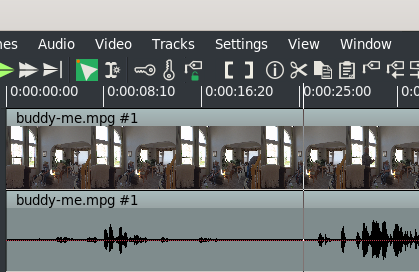
\includegraphics[width=0.6\linewidth]{images/insertion-point.png}};
        \node [yshift=-13mm, xshift=-1cm,anchor=east] at (img1.north west) (Pulldowns) {Pulldowns};
        \node [yshift=-20mm, xshift=-1cm,anchor=east] at (img1.north west) (Transport) {Transport \& Buttons Bar};
        \node [yshift=-27mm, xshift=-1cm,anchor=east] at (img1.north west) (Timebar) {Timebar};
        \node [yshift=-33mm, xshift=-1cm,anchor=east] at (img1.north west) (Title) {Media Title };
        \node [yshift=-43mm, xshift=-1cm,anchor=east] at (img1.north west) (Video) {Video Track};
        \node [yshift=-63mm, xshift=-1cm,anchor=east] at (img1.north west) (Audio) {Audio Track};
        \draw [->, line width=1mm] (Pulldowns) edge  ([yshift=-13mm] img1.north west);
        \draw [->, line width=1mm] (Transport) edge  ([yshift=-20mm] img1.north west);
        \draw [->, line width=1mm] (Timebar) edge    ([yshift=-27mm] img1.north west);
        \draw [->, line width=1mm] (Title) edge      ([yshift=-33mm] img1.north west);
        \draw [->, line width=1mm] (Video) edge      ([yshift=-43mm] img1.north west);
        \draw [->, line width=1mm] (Audio) edge      ([yshift=-63mm] img1.north west);
        \end{tikzpicture}
    
    \caption{Insertion point is at 0:00:25:10 in Hr:Mn:Sec:Frames}
    \label{fig:insertion-points}
\end{figure}


\subsection{Editing Modes}%
\label{sub:editing_modes}

There are 2 different editing methods of operation that affect the insertion point and the editing on the timeline.  
There is:  \emph{drag and drop mode} and \emph{cut and paste mode}. 
The editing mode is determined by selecting the arrow or the I-beam in the Transport and Buttons bar. 

If the arrow is highlighted, it enables \emph{drag and drop mode}.  
In drag and drop mode, clicking in the timeline does not reposition the insertion point.  
Double-clicking in the timeline selects the entire edit the mouse pointer is over.  
Dragging in the timeline repositions the edit the mouse pointer is over. 
This is useful for reordering audio playlists, sorting movie scenes, or moving effects around. 
To cut and paste in drag and drop mode you need to set in/out points to define an affected region. 

If the I-beam is highlighted it enables \emph{cut and paste mode}. 
In cut and paste mode, clicking in the timeline repositions the insertion point. 
Double-clicking in the timeline selects the entire edit the cursor is over. 
Dragging in the timeline highlights a region. 
The highlighted region becomes the region affected by cut and paste operations and the playback range during the next playback operation. 
Shift-clicking in the timeline extends the highlighted region.

When highlighting a region, the start and end points are either aligned to frames or aligned to samples. When editing video, you will want to align to frames. When editing audio you will want to align to samples. Select your preference by using settings$\rightarrow$align cursor on frames.

\begin{figure}[htpb]
    \centering
    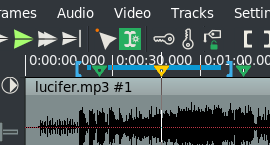
\includegraphics[width=0.4\linewidth]{images/i-beam.png}
    \caption{I-beam + in/out  +  labels}
    \label{fig:i-beam}
\end{figure}

\subsection{In/Out Points}%
\label{sub:in_out_points}

In both editing modes, you can set one In point and one Out point. 
The in/out points define the affected region. 
In drag and drop mode, they are the only way to define an affected region. 
In both cut and paste mode and drag and drop mode, the highlighted area overrides the In/Out points. 
If a highlighted area and In/Out points are set, the highlighted area is affected by editing operations and the In/Out points are ignored. 
If no region is highlighted, the In/Out points are used. 
To avoid confusion, it is better to use either highlighting or In/Out points but not both simultaneously.

To set in/out points, go to the timebar and position the insertion point somewhere. 
Select the In point button. 
Move the insertion point to a position after the In point and click the Out point button. 
Instead of using the button bar, you can use the [ or < and ] or > keys to toggle in/out points.

If you set the insertion point somewhere else while In/Out points already exist, when you click the In/Out buttons the existing points will be repositioned. 
If you click on in/out points while a region is highlighted, the insertion point will be ignored and In/Out points will be set at the beginning and at the end of the highlighted area.

If you select either the In point or the Out point, the insertion point will jump to that location. 
After selecting an In point, if you click the In point button the In point will be deleted. 
After selecting an Out point, if you click the Out point button the Out point will be deleted. 
Shift-clicking on an In/Out point highlights the region between the insertion point and that In/Out point. 
If a region is already highlighted, it extends the highlighted region up to that In/Out point.

To quickly get rid of In/Out points, without caring about where they are or if they are set or not, just double click on [ and ] buttons. 
The first click will set a new point or reposition an old one at the insertion point; the second click will delete it. This trick does not work if the In point or the Out point is already set at insertion point.

Some of the useful operations concerning the In/Out pointers are listed next.

\begin{description}
    \item[Ctrl-KeyPad\#]  if in/out set, KP 2,3,5,6 + Enter, play between In/Out point
    \item[Shift-Ctrl]  loops play between In/Out points
    \item[Click in/out] while holding the left mouse button, drags In/Out pointer elsewhere
    \item[Shift-Ctrl] with transport button, loops play between In/Out points
    \item[Ctrl-t]  clears both In/Out points
\end{description}

\subsection{Labels}%
\label{sub:labels}

The insertion point and the In/Out points allow you to define an affected region, but they do not let you jump to exact points on the timeline very easily. 
Labels are an easy way to set exact locations on the timeline that you want to jump to. 
When you position the insertion point somewhere and click the label button, a new label appears on the timeline. 
With label traversal you can quickly seek back and forth on the timeline.

No matter what the zoom settings are, clicking on the label highlights it and positions the insertion point exactly where you set the label. 
The lower case letter “L” is a shortcut for the label button.

Labels can reposition the insertion point when they are selected but they can also be traversed with the label traversal buttons. When a label is out of view, the label traversal buttons reposition the timeline so the label is visible. Keyboard shortcuts for label traversal are:

\begin{description}
    \item[Ctrl-left] repositions the insertion point on the previous label.
    \item[Ctrl-right] repositions the insertion point on the next label.
\end{description}

The Label folder in the Resources window lists the timestamp of every label. 
You can edit the label list and add a title for every item using the popup menu. 
To open the Label info dialog right click on the label icon in the Resources window or directly on the label symbol on the timebar. 
With labels you can also select regions:

\begin{description}
    \item[Shift-Ctrl-left] highlights the region between the insertion point and the previous label.
    \item[Shift-Ctrl-right] highlights the region between the insertion point and the next label.
    \item[Double-clicking] on the timebar between two labels highlights the region between the labels.	   
    \item[Shift-clicking] on a label highlights the region between that label and the insertion point.
        If a region is already highlighted, it extends the highlighted region up to that label.
\end{description}


If you hit the label button when a region is highlighted, labels are created at each end of the highlighted region. 
However, if one end already has a label, then the existing label is deleted. 
Hitting the label button again when a label is selected deletes it. 
Manually hitting the label button or L key over and over again to delete a series of labels can get tedious. 
To delete a set of labels, first highlight a region, then use the Edit$\rightarrow$Clear labels function. 
If in/out points exist, the labels between the in/out points are cleared and the highlighted region is ignored.


In Cut and Paste editing mode only, by enabling \emph{Edit labels} in the settings menu or by disabling the \emph{Lock labels from moving} button on the program toolbar, labels will be cut, copied or pasted along with the selected region of the first armed track. 
Similarly, if a selected area of a resource is spliced from the viewer to the timeline in a position before labels, these labels will be pushed to the right on the timebar for the length of the selected area. 
To prevent labels from moving on the timebar, just disable the \emph{Edit labels} option or enable the \emph{Lock labels from moving} button.


Originally in Drag and Drop editing mode labels will be always locked to the timebar, even with the \emph{Edit labels} option enabled.  
This may no longer be correct in all cases. 

\subsection{Color Title Bars and Assets}%
\label{sub:color_title_bars_and_assets}

In order to visually aid in locating clips on the timeline that are from the same media file, you can have them auto-colored or self-colored.  
Use of this feature requires additional memory and cpu on every timeline redraw, therefore it is recommended that smaller computers leave it turned off.

For auto-color the color will be based on a hashed filename so that whenever you load this particular media, it will always have the same color on the title bar even if you use proxy.  
To enable auto-color (figure~\ref{fig:autocolor_assets}, go to Settings$\rightarrow$Preferences, Appearance tab and check on “Autocolor assets”.  
It is disabled by default.  
Each media will have a random muted color and there could easily be close duplicates as generated by the program algorithm.  There will be no total black, but some dark shades are possible.  

Screencast shows the red colored checkmark to enable Autocolor assets.  
In the lower left corner is Highlighting Inversion color which can also be set and is discussed elsewhere.

\begin{figure}[htpb]
    \centering
    \includegraphics[width=0.8\linewidth]{images/autocolor-assets.png}
    \caption{Autocolor assets}
    \label{fig:autocolor_assets}
\end{figure}

To change a specific clip to your own chosen color, middle mouse button over that clip and an Edits popup will be displayed.  
Choose the option \emph{Bar Color} to bring up the color picker and choose a color.   
You can also change the alpha value in the color picker and this alpha takes precedence over the current alpha slider bar value unless it was set to 1.0.   
The color will only change after you click on the checkmark.  
The \emph{Bar Color} option works in either Drag and Drop or Cut and Paste editing mode and also works if “Autocolor assets” is not set.  
In Drag and Drop editing mode, if you select several clips and then bring up the Edits popup with the middle mouse button over a track, you can use the \emph{Bar Color} option to change all of those selected to the same color.

To go back to the default colors, uncheck “Autocolor assets” in Preferences, but this does not affect the specially chosen self-colored ones as they are preserved.  
To change these individually or  selectively use the Edits popup \emph{Bar Color} option and click on “Default” in the color picker window.  Auto-color does not honor armed/disarmed tracks.  
Self-color does honor armed/disarmed tracks.

And that’s not all!  
There is an \emph{alpha fader slider bar} on the bottom of the main window on the right hand side of what is referred to as the Zoom Panel.  
With this alpha slider, you can colorize your video and audio tracks to either see only the color at 0.0 or see only the image/audio waveform at 1.0.  
This slider bar affects all colored areas of the Autocolor assets and the self-colored ones.  
In the case when a specifically changed edit alpha value is any value except 1, the slider bar will not affect that.  
Once you use the slider bar, it is activated so gets first shot at any keystrokes in the main window.  
You deactivate this by simply clicking in a different part of the main window.  

As long as we are on the subject of color, just a reminder that you can also change the “Highlighting Inversion color” in Settings$\rightarrow$Preferences, Appearance tab.  
This is on right left hand side of the menu more than half the way down and you can see this in the figure~\ref{fig:autocolor_assets}.  
That setting defaults to white (ffffff) but sometimes this is a little bright so you can put any hex value in that suits you.

Screencast (figure~\ref{fig:autocolor_assets_alpha}a) which shows an example of the Autocolor assets with alpha set to 0.0.
In this screencast (figure~\ref{fig:autocolor_assets_alpha}b), the alpha is set to show the image as well as the colors.  The pink media file has been self-colored rather than the autocolor to make it easy to see.

\begin{figure}[htpb]
    \centering
    \begin{minipage}[h]{0.55\linewidth}
        \center{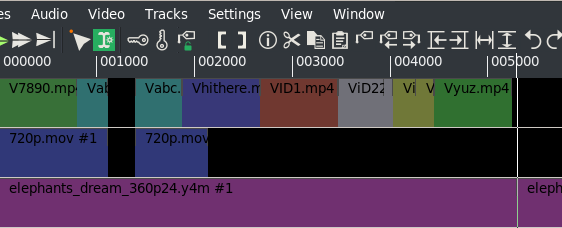
\includegraphics[width=0.99\linewidth]{images/autocolor-assets_alpha0.png}} \\ a)
    \end{minipage}
    \begin{minipage}[h]{0.4\linewidth}
        \center{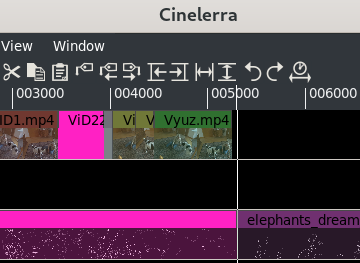
\includegraphics[width=0.99\linewidth]{images/autocolor-assets_alpha1.png}} \\ b)
    \end{minipage}
    \caption{An example of the Autocolor assets}
    \label{fig:autocolor_assets_alpha}
\end{figure}


\subsection{More about Pulldowns}%
\label{sub:more_about_pulldowns}

The main window pulldowns are quite obvious in their meaning and usage, so here is only a summary.  
%TODO Figure 3 shows an example of the pulldowns as displayed in the main window.


\begin{description}
    \item[File]  options for loading, saving, and rendering as described in other sections.
    \item[Edit]  edit functions; most of which have shortcuts that you will quickly learn.
    \item[Keyframes]  keyframe options which are described in the Keyframe section.
    \item[Audio]  audio related functions such as “Add track”, “Attach transition/effect”.
    \item[Video]  video functions such as “Default/Attach transition”.
    \item[Tracks]  move or delete tracks are the most often used.
    \item[Settings]  this is mostly described in other sections.  
        However, typeless keyframes are not described
        anywhere else.  
        They allow keyframes from any track to be pasted on either audio or video tracks.
    \item[View]  for display or modifying asset parameters and values to include Fade, Speed, and Cameras.
    \item[Window]  window manipulation functions.
\end{description}


\subsection{Window Layouts}%
\label{sub:window_layouts}

If you like to use different window layouts than the default for certain scenarios, you can setup, save, and load 4 options.   
First position your Cinelerra windows where you want them to be and then use the Window pulldown and choose \emph{Save layout}.  
To use the default name of Layout \#, when the popup comes up, just click the green checkmark OK on the Layout popup menu.  
If you would like a specific name for your layout so you can remember what it is for, keyin 1-8 english characters that are meaningful to you (english characters mean you can not use the German umlaut or the French accent).  
Legal characters are a-z, A-z, 0-9, \_ (the underscore character) and a limit of 8 total.  
If you keyin more than 8, only the last 8 characters will be used.  
To rename a currently existing layout, use the Save layout option again on the one to rename, and keyin a different name into the text box or blank for the default name (figure~\ref{fig:window_layouts}).

\begin{figure}[htpb]
    \centering
    \begin{minipage}{.49\linewidth}
        \center{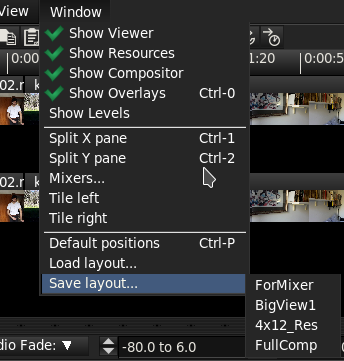
\includegraphics[width=1\linewidth]{images/window_layout1.png}}\\ a)
        %TODO High res image replace
    \end{minipage}
    \begin{minipage}{.49\linewidth}
        \vspace{13ex}
        \center{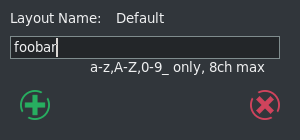
\includegraphics[width=1\linewidth]{images/window_layout2.png}}\\ b)
        %TODO Alpha channel
    \end{minipage}
    \caption{Window Layouts}
    \label{fig:window_layouts}
\end{figure}

The files containing the coordinates for your layouts will automatically be saved in the \texttt{\$HOME/.bcast} directory as \texttt{layout\#\_rc} or \texttt{layout\#\_8chars\_rc}.

To use the desired layout, keyin the shortcut or use the Window pulldown and choose \emph{Load layout} and then make your choice. 

\subsection{Just Playing!}%
\label{sub:just_playing_}
What if you are just using Cinelerra to play media and listen to tunes? 
After loading your media, just hit the space bar to start playing and then again to stop playing.  
Other than that, use the transport buttons on the top bar of the Program window.  
Other ways, not previously mentioned to “play around” are described next. 

\subsubsection*{Repeat Play / Looping Method}%
\label{ssub:repeat_play_looping_method}

There are 2 methods for repeat play or looping on the timeline and 1 method for both the Compositor and the Viewer.  This works in conjunction with any of the transport buttons or shortcuts in either forward or reverse as usual.  The 1 exception is that the Shift button can not be used to either add or subtract audio within the repeat area.


\emph{Shift-L on the Timeline}, repeats the selection per the algorithm outlined next.  
When setup, long green lines are displayed across the entire set of tracks which shows the start and end of the loop.
\begin{enumerate}
    \item  Highlighted selection repeats loop and takes precedence over all other possibilities.  
        If the cursor is before the highlighted area, it will play up to the area and then repeat the highlighted section.  
        If the cursor is after the highlighted section, play will start at the beginning until you get to the
        highlighted section and then repeat.
    \item  When both In and Out pointers are set, it repeats the section between [ and ].
    \item  If only one of the In or Out pointers is set, it loops the whole media.
\end{enumerate}

\emph{Ctrl+Shift+transport button on the Timeline, Viewer, and Compositor}

\begin{enumerate}
    \item Repeats entire media if no In or Out pointer set.
    \item  In and Out pointer set, repeats area between pointers.
    \item  Only In pointer set, repeats from In to end of media.
\end{enumerate}

\subsubsection*{Last Play Position Memory}%
\label{ssub:last_play_position_memory}


When you play media, the start/end playback positions are saved as if they had been made into temporary labels.  
They appear on the timeline as purple/yellow hairline markers representing the last start/end labels for the last playback. 
They can be addressed as if they are label markers using:

\begin{description}
    \item[Ctrl$\leftarrow$]   tab to the label before the cursor, that is “play start”
    \item[Ctrl$\rightarrow$]   tab to the label after the cursor, that is “play stop”
\end{description}


You can use these markers for re-selection.  
Additionally, the selection region can be expanded by “pushing” the markers using single frame playback.  
Use frame reverse (keypad 4) to push the start play marker backward, or use frame forward (keypad 1) to push the end play marker forward.

Another handy feature is to use the combination of Ctrl-shift-arrow (left or right) to select the media from the cursor position (red hairline) to the start or end marker by “tabbing” to the label markers.  
For example, tab to the beginning of the previous play region using Ctrl-left-arrow to move the cursor to the beginning of last play, then press Ctrl-Shift-right-arrow to tab to the end of the playback region. 
Now you can clip/play/expand or edit the previous playback selection.

\begin{description}
    \item[Ctrl SHIFT$\rightarrow$] 	  tab cursor to label right of cursor position and expand selection
    \item[Ctrl SHIFT$\leftarrow$] 	  tab cursor to label left of cursor position and expand selection
\end{description}


\subsubsection*{Playback Speed Automation Support}%
\label{ssub:playback_speed_automation_support}


The speed automation causes the playback sampling rate to increase or decrease to a period controlled by the speed automation curve.  
This can make playback speed-up or slow-down according to the scaled sampling rate, as “time is multiplied by speed” (speed X unit\_rate).

\subsubsection*{Alternative to using Numeric Keypad for Playing}%
\label{ssub:alternative_to_using_numeric_keypad_for_playing}


For the keyboards without a numeric keypad or if you prefer to use keys closer to where you normally type, there are alternative keys for the play/transport functions.  These are listed below.

\begin{tabular}{lcl}
	Alt + m&=&stop playback\\

	Alt + j&=&forward single frame\\

	Alt + k&=&forward slow playback\\

	Alt + l&=&forward normal playback\\

	Alt + ;&=&forward fast playback\\

	Alt + u&=&reverse single frame\\

	Alt + i&=&reverse slow playback\\

	Alt + o&=&reverse normal playback\\

	Alt + p&=&reverse fast playback\\
\end{tabular}
\begin{minipage}{.45\linewidth}
+ Shift key, results in the reverse of whether audio is included or not.
\vspace{1ex}

+ Ctrl, results in the transport function operating only between the in/out pointers.
\end{minipage}

\section{Compositor Window}%
\label{sec:compositor_window}

The Compositor window (figure~\ref{fig:compositor_window}) displays the output of the timeline. 
It is the interface for most compositing operations or operations that affect the appearance of the timeline output. 
Operations done in the Compositor affect the timeline but do not affect clips.

\begin{figure}[htpb]
    \centering
    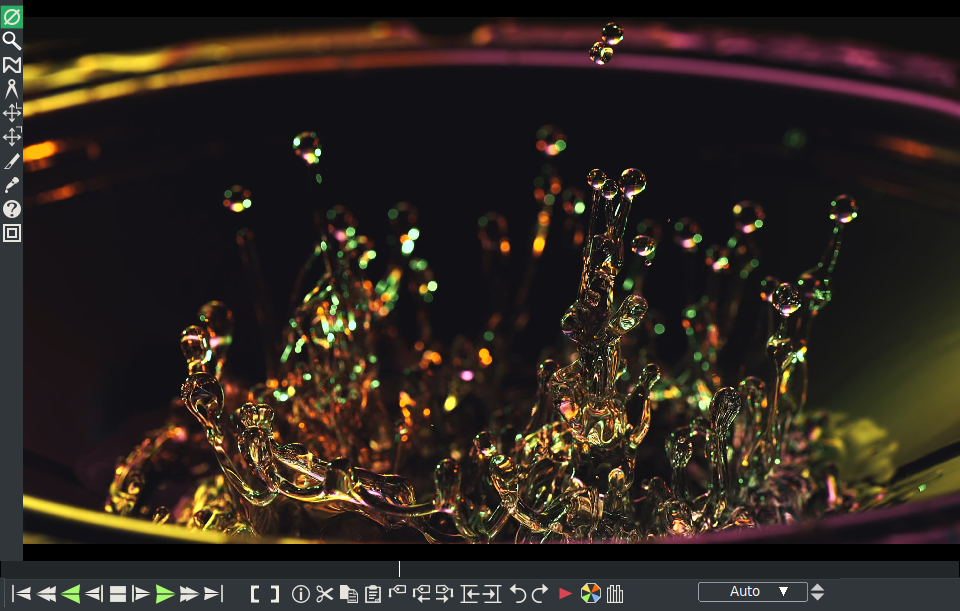
\includegraphics[width=0.99\linewidth]{images/compositor_window.png}
    \caption{Upper right side contains navigation tools / bottom bar has manu control functions}
    \label{fig:compositor_window}
\end{figure}

\subsection{Compositor controls}%
\label{sub:compositor_controls}


Navigating the video output does not affect the rendered output; it just changes the point of view in the compositor window. 
The video output has several navigation functions. 
The video output size is either locked to the window size or unlocked with scrollbars for navigation. 
The video output can be zoomed in and out and panned. 
If it is unlocked from the window size, middle clicking and dragging anywhere in the video pans the point of view. Hitting the + and - keys zooms in and out of the video output.

Underneath the video output are copies of many of the functions available in the main window. 
In addition there is a zoom menu and a tally light. 
The zoom menu jumps to all the possible zoom settings and, through the Auto option, locks the video to the window size. 
The zoom menu does not affect the window size. 
The tally light turns red when rendering is happening. This is useful for knowing if the output is current. 
Right clicking anywhere in the video output brings up a menu with all the zoom levels, zoom auto mode, and some other options. 
In this particular case the zoom levels resize the entire window and not just the video. 
The \emph{Reset camera} and \emph{Reset projector} options center the camera and projector. 
The \emph{Hide controls} option hides everything except the video. 

On the left of the video output is a toolbar specific to the compositor window. The toolbar has the following functions:

\emph{Protect video} --- disables changes to the compositor output from clicks in it. It is an extra layer on top of the track arming toggle to prevent unwanted changes.

\emph{Magnifying glass} --- this tool zooms in and out of the compositor output without resizing the window. If the video output is currently locked to the size of the window, clicking in it with the magnifying glass unlocks it and creates scrollbars for navigation.

\begin{description}
    \item[Left clicking] in the video zooms in;
    \item[Ctrl clicking] in the video zooms out;
    \item[Rotating the wheel] on a wheel mouse zooms in and out.
\end{description}

In addition, if you enable the Magnifying glass, a zoom slider for fine-viewing appears below these tools.  
It allows you to zoom to most any size. 
A “zoom slider” will pop-up towards the bottom on the left-hand side of the Compositor when you enable “Zoom view” via the magnifying glass or when you click on the icons for “Adjust camera automation” or “Adjust projector automation”.  
This will allow for adjusting the amount of zoom at any level between 0.01 and 100 based on a logarithmic scale.  
When using the zoom slider, the number by which the view is zoomed can be seen in the textbox where the original-also-working \% zoom is located.  
The zoom slider size is in the form of “times”, such as x 0.82 which indicates that the picture is zoomed to 82/100th of the original size as seen in Settings$\rightarrow$Format.  
Once you have set the zoom to the desired size, use the vertical and horizontal scroll bars to position the view as needed.

Screencast (figure~\ref{fig:zoom_slider}) shows below at a zoom slider bar with the diamond shaped slider in the middle.  Note 
that the magnifying glass is  enabled which automatically pops-up the slider.

\begin{figure}[htpb]
    \centering
    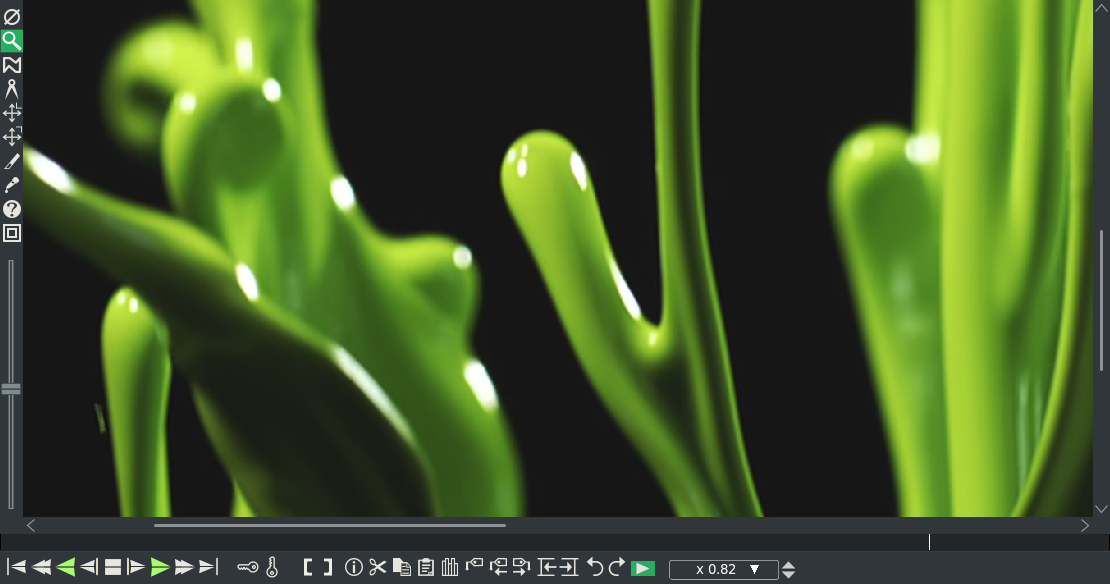
\includegraphics[width=0.99\linewidth]{images/zoom_slider.png}
    \caption{A zoom slider bar with the diamond shaped slider in the middle}
    \label{fig:zoom_slider}
\end{figure}
The Format shows a large 5204x3468 video and the box at the arrow shows x 0.82 size.  

\begin{description}
    \item[Masks tool] this tool brings up the mask editing tool. Enable “Show tool info” to see the options.
    \item[Camera]  the camera brings up the camera editing tool. Enable “Show tool info” to see options.
    \item[Projector]  the projector brings up the projector editing tool. Enable “Show tool info” for options.
    \item[Crop tool]  this tool brings up the cropping tool. “Show tool info” must be enabled to use this tool.
    \item[Eyedropper]  brings up the eyedropper. The eyedropper detects whatever color is under it and stores it
        in a temporary area. Enabling the “Show tool info” shows the currently selected color. Click
        anywhere in the video output to select the color at that point. The eyedropper not only lets you see
        areas which are clipped, but its value can be applied to many effects. Different effects handle the
        eyedropper differently.
    \item[Show tool info]  this tool button works only in conjunction with the other controls on the compositor.
        Based on what compositing control is active, the toggle button will activate or deactivate the
        appropriate control dialog box. Controls with dialog boxes are: Edit mask, Camera and Projector
        automation, Crop control, and Get color.
    \item[Safe regions tool]  draws the safe regions in the video output. The largest (external) square is called \textit{action safe overlay}; the smallest internal square is called \textit{title safe overlay}. They are especially useful if the destination is the TV. This does not affect the rendered output
\end{description}

\subsection{Compositing}%
\label{sub:compositing}

A large amount of Cinelerra's editing is directed towards compositing. 
Changing the resolution of a show, making a split screen, and fading in and out among other things are all compositing operations in Cinelerra. 
Cinelerra detects when it is in a compositing operation and plays back through the compositing engine only then. 
Otherwise, it uses the fastest decoder available in the hardware.

Compositing operations are done on the timeline and in the Compositor window. Shortcuts exist in the Resource window for changing some compositing attributes. 
Once some video files are on the timeline, the compositor window is a good place to try compositing.

\subsection{Camera and Projector}%
\label{sub:camera_and_projector}

In the compositor window, two of the more important functions are the adjust camera automation and the adjust projector automation which control operation of the camera and projector. 
Cinelerra's compositing routines use a \textit{temporary}, a frame of video in memory where all graphics processing is performed. 
Inside Cinelerra's compositing pipeline, the camera determines where in the source video the \textit{temporary} is copied from. 
The projector determines where in the output the \textit{temporary} is copied to (figure~\ref{fig:temporary-01}). 
Each track has a different \textit{temporary} which is defined by the track size. By resizing the tracks you can create split screens, pans, and zooms.

\begin{figure}[htpb]
    \centering
    \includegraphics[width=0.8\linewidth]{images/temporary-01.pdf}
    \caption{Compositing pipeline}
    \label{fig:temporary-01}
\end{figure}

In compositing, each frame can be digitally altered using various options, such as a color correction plugin (figure~\ref{fig:camera_and_projector}). 
Once the image has been transformed, the finished image is then projected to the compositor thus creating a modified version of the original.

\begin{figure}[htpb]
    \centering
    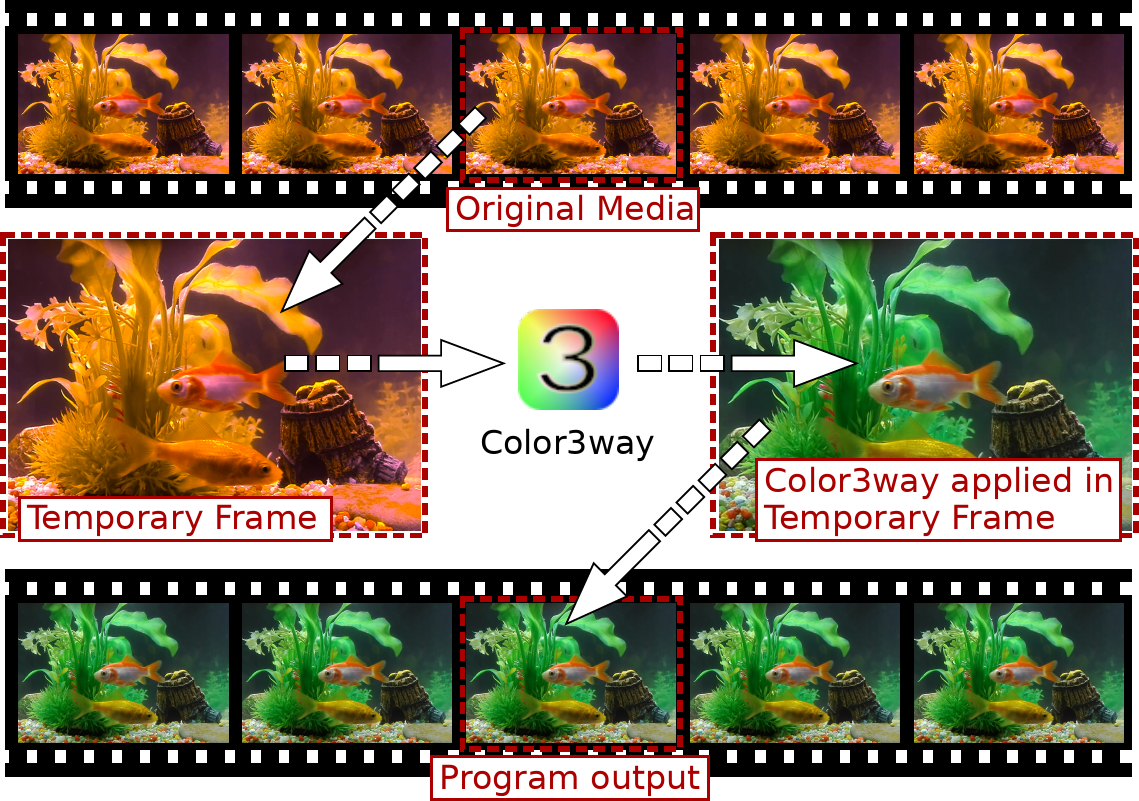
\includegraphics[width=0.8\linewidth]{images/camera_and_projector.png}
    \caption{Color balance on Temporary}
    \label{fig:camera_and_projector}
\end{figure}

When editing the camera and projector in the compositing window, the first track with record enabled is the track affected. 
Even if the track is completely transparent, it is still the affected track. 
If multiple video tracks exist, the easiest way to select one track for editing is to Shift-click on the record icon of the track. 
This solos the track.

The purpose of the projector is to place the contents of the \textit{temporary} into the project's output.  
The intent of the projector is to composite several sources from the various tracks into one final output track. 
The projector alignment frame is identical to the camera's viewport, except that it guides where on the output canvas to put the contents of each temporary.

\subsubsection*{Compositing projector controls}%
\label{ssub:compositing_projector_controls}

When the projector button is enabled in the compositor window, you are in projector editing mode. A guide box appears in the video window. The red box indicates the size of the frame that will be sent to the Ouput. You can drag the box with LMB, moving the frame in x and y as you like. Even when moving along the z-axis (i.e. the zoom, with SHIFT+Drag) the red box faithfully follows the movement and size of the frame. Once you have positioned the video with the projector, you may want to work with adjusting the camera automation.

\subsubsection*{Viewport sizes}%
\label{ssub:viewport_sizes}

The viewport is a window on the camera that frames the area of source video to be scanned.
The initial size of the viewport is defined by the size of the current track. A smaller viewport (640x400) captures a smaller area. 
A larger viewport (800x200) captures an area larger than the source video and fills the empty spaces with blanks. 
Once we have our viewport defined, we still need to place the camera right above the area of source video we are interested on. To control the location of the camera:

\begin{enumerate}
    \item  Open the compositor window with a track selected.
    \item  Select the camera button to enable camera editing mode.
    \item  Drag over the display window.
\end{enumerate}

When we drag over the viewport in the compositor window, the way it looks is as if you \textit{move the camera with the mouse}.  The viewport also moves with it.

\subsubsection*{Compositing camera controls}%
\label{ssub:compositing_camera_controls}

Select the camera button to enable camera editing mode. 
In this mode, the guide box shows where the camera position is in relation to past and future camera positions but not where it is in relation to the source video. 
The green box is the Viewport; at the beginning it coincides with the size of the source frame. If we move the viewport by dragging it with LMB (moving it in x/y), the green box remains fixed to the original size but the frame is moved to the new position.  A yellow frame will appear along the edges of the frame to indicate the displacement with respect to the green box; this behavior differs from that seen for the Projector. Even if we act on the z-axis (SHIFT + Drag, equivalent to the zoom), the frame narrows or widens, moving behind the yellow frame.

\subsubsection*{The camera and projector tool window}%
\label{ssub:the_camera_and_projector_tool_window}

The camera and projector have shortcut operations that do not appear in the popup menu and are not represented in video overlays. 
These are accessed in the \emph{Show tool info} window . 
Most operations in the Compositor window have a tool window which is enabled by activating the question mark icon (figure~\ref{fig:camera_tool}).

\begin{wrapfigure}[12]{O}{0.3\linewidth} 
	\vspace{-2ex}
    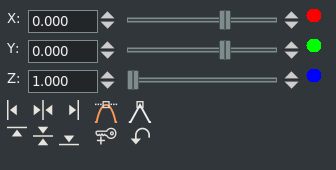
\includegraphics[width=0.9\linewidth]{images/camera_tool.png}
    \caption{Camera and Projector tool}
    \label{fig:camera_tool}
\end{wrapfigure}

In the case of the camera and projector, the tool window shows x, y, and z coordinates. 
By either tumbling or entering text directly, the camera and projector can be precisely positioned.  
Justification types are also defined for easy access. 
A popular justification operation is upper left projection after image reduction. 
This is used when reducing the size of video with aspect ratio adjustment.  
In the last figure you see the choices for justification as the red stripe in the 6 boxes in the order of left, center horizontal, right, top, center vertical, and bottom.

The translation effect allows simultaneous aspect ratio conversion and reduction but is easier to use if the reduced video is put in the upper left of the \textit{temporary} instead of in the center. 
The track size is set to the original size of the video and the camera is centered. 
The output size is set to the reduced size of the video. 
Without any effects, this produces just the cropped center portion of the video in the output.

The translation effect is dropped onto the video track. The input dimensions of the translation effect are set to the original size and the output dimensions are set to the reduced size. 
To put the reduced video in the center subsection that the projector shows would require offsetting out x and out y by a complicated calculation. 
Instead, we leave out x and out y at 0 and use the projector's tool window. 
By selecting left justify and top justify, the projector displays the reduced image from the top left corner of the \textit{temporary} in the center of the output.

\subsubsection*{Reset to Default}%
\label{ssub:reset_default}

In the compositing window, there is a popup menu of options for the camera and projector. Right click over the video portion of the compositing window to bring up the menu:

\texttt{Reset Camera}: causes the camera to return to the center position.
    	
\texttt{Reset Projector}: causes the projector to return to the center.

\subsubsection*{Use Case: Interaction Between Camera And Projector \protect\footnote{Example provided by Sam. The relative video is located at: \url{https://streamable.com/iq08i}}}%
\label{ssub:use_case_interaction_camera_projector}

\begin{enumerate}
    \item Start by shrinking the projector to "z=0,500" ($\frac{1}{4}$ of the original frame).
    \item The next step is to switch to the camera and note that the green box has assumed the size of the projector, i.e. the red box. The value of z of the camera is always equal to $1,000$ (default) but the frame is $\frac{1}{4}$ of the original frame, i.e. it has the size of the projector that has $z=0,500$. This is the current viewport size.
    \item You enlarge the room bringing $z=2,000$. You can see that the dimensions of the viewport (green box) do not change, remaining the same as those of the projector. However, the frame has been enlarged and this variation is indicated by the enlargement of the yellow box. Let's remember that this follows the changes made with the camera tool.
    \item We can drag the room so that we can center the frame to our liking. . The movement of the yellow box shows well the variation compared to the green box.
    \item Finally, if we want, we can switch to the projector tool to move the output frame to the position we want with respect to the size of the source. Of course, we can also work on the z, which in the example is at $z=0.500$, if we have decided to change the size of the output.
\end{enumerate}

\subsection{Masks}%
\label{sub:masks}

Masks select a region of the video for either displaying or hiding. 
Masks are also used in conjunction with another effect to isolate the effect to a certain region of the frame. 
A copy of one video track may be delayed slightly and unmasked in locations where the one copy has interference but the other copy does not. 
Color correction may be needed in one subsection of a frame but not another. 
A mask can be applied to just a subsection of the color corrected track while the plain track shows through. 
Removal of boom microphones and airplanes are a common kind of mask uses.

The order of the compositing pipeline affects what can be done with masks. Mainly, masks are performed on the temporary after effects and before the projector. This means multiple tracks can be bounced to a masked track and projected with the same mask.

The compositing pipeline graph has a masking stage (figure~\ref{fig:temporary-02}).

\begin{figure}[htpb]
    \centering
    \includegraphics[width=0.7\linewidth]{images/temporary-02.pdf}
    \caption{compositing pipeline with mask}
    \label{fig:temporary-02}
\end{figure}

There are 8 possible masks per track. Each mask is defined separately, although they each perform the same operation, whether it is addition or subtraction.

\subsubsection*{Compositing pipeline with masks}%
\label{ssub:compositing_pipeline_with_masks}

\begin{enumerate}
    \item To define a mask, go into the Compositor window and enable the mask toggle.
    \item  Next go over the video and click-drag. 
        Note: You have to select automatic keyframes if you wish to move a mask over time.  
        If you do not, the mask position will be the same even if you edit at different places on the timeline.
    \item  Click-drag again in another part of the image to create each new point of the mask. 
        While it is not the conventional Bezier curve behavior, this masking interface performs in realtime what the effect 
        of the mask is going to be. Creating each point of the mask expands a rubber band curve.

        Once points are defined, they can be moved by Ctrl-dragging in the vicinity of the corner. 
        Shift-drag allows you to move existing points to new locations, thus altering the shape of the mask.  
        However, this does not smooth out the curve. 
        The In/Out points of the Bezier curve are accessed by Ctrl-dragging in the vicinity of the corner. 
        Then Ctrl-dragging near the In or Out point causes the point to move.  
        Shift-drag activates bezier handles to create curves between mask points.       

    \item  Finally once you have a mask, the mask can be translated in one piece by Alt-dragging the mask.
    The effect of the mask is always on.  
    Ctrl-Alt-drag translates an entire mask to a new location on the
    screen.
\end{enumerate}

The masks have many more parameters which could not be represented with video overlays. 
These are represented in the tool window for masks. 
Selecting the question mark when the mask toggle is highlighted brings up the mask options window (figure~\ref{fig:mask_window}).

\begin{figure}[htpb]
    \centering
    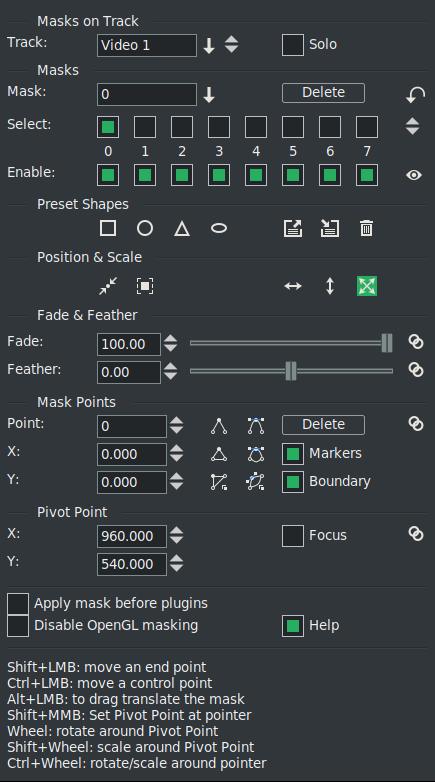
\includegraphics[width=0.6\linewidth]{images/mask_window.png}
    \caption{Mask options window}
    \label{fig:mask_window}
\end{figure}

Masking has been greatly improved compared to the original tool.  Detailed description is provided here.  Note that the Mask window is separated into various sections to make it easier to locate the area of interest.

\subsubsection*{Masks on Track section}%
\label{ssub:masks_track_section}

The \texttt{Track}: textbox displays the different video tracks for your session which will be initially set to the first armed video track or will be left blank if there are no armed tracks.  A pulldown to the right of the box brings up the names of all of the video tracks allowing you to change to which track the masking applies.  You can also just use the tumbler to easily mouse up/down to get to the desired track. In the pulldown list, any track that has red colored text is disarmed so that you can not change it.  A track that contains masks has yellow colored text for easy identification.  Only when there are no masks on the track, do you have the default text color. This textbox is display only and you can not type into it.

The \texttt{Solo} button in the Masks on Track section of the Mask window is very handy when working with masks on different tracks.  It displays only that track so that you only see the track you choose, as well as the tracks behind it to show the mask part.  The Solo button is just a convenience to prevent having to mouse over to the patchbay.

\subsubsection*{Masks section}%
\label{ssub:masks_section}

The \texttt{Mask}: textbox will show you the mask numbers of $0-7$ or the 8 ascii character name that you have used to designate each mask number.  There is a pulldown on the right side to easily switch to another mask. 

The \texttt{Delete} button is used to delete the mask number/name that is selected. The symbol to the right with tooltip of \texttt{Delete all masks} can be used to delete all of the current video track masks.

The \texttt{Select}: row of checkboxes is used to indicate which mask is currently displayed for that video track in the Compositor.  Numbers that are colored yellow are active masks for that track.  A tumbler to the right allows for quickly changing the mask number displayed.

The \texttt{Enable} row of masks makes it so you can enable all or none of the masks, making it possible to look at no masks or at one mask without interference from the other masks. The symbol that looks like an \texttt{eye} can be used to easily check all or none as the tooltip \textit{Show/Hide mask states}.

\subsubsection*{Preset Shapes section}%
\label{ssub:preset_shape_section}

There are 4 shapes that are automatically available for usage as masks – \texttt{square}, \texttt{circle}, \texttt{triangle}, and \texttt{oval}.  In addition, the next 3 symbols in this section are for the purpose of loading, saving, and deleting your own customized shapes.  The first symbol, \texttt{Load} preset, will bring up a list of your previously saved presets.  Clicking on \texttt{Save} preset brings up a popup window allowing you to provide a name used to identify the preset you want to save, along with a pulldown to see the names of your other saved presets.   Clicking on \texttt{Delete} preset also brings up a textbox with a pulldown to choose which one to delete.  There is a file, called \texttt{mask\_rc}, in \texttt{\$HOME/.bcast5} that records your custom masks.  

When you click \texttt{Load} preset, keep in mind that it will write the mask number that you have selected so if you already have a mask at that location, it will write over it – just UNDO to revert to the previous if you made this mistake.

\subsubsection*{Position \& Scale section}%
\label{ssub:position_scale_section}

\texttt{Center} mask button allows for quickly centering a mask on the video track. 
\texttt{Normalize} mask button makes it easy to normalize the size of the mask based on the scale of the video. 
The next 3 symbols concern the direction to \textit{drag translate} a mask using the \texttt{Alt+Left Mouse Button} thus making it easy to preserve the current $X$ or $Y$ value when desirable.

\texttt{xlate/scale x}	- drag translate constrained in the X direction

\texttt{xlate/scale y}	- drag translate constrained in the Y direction

\texttt{xlate/scale x/y}	- drag translate in both directions; this is the default and after using the other 2 options, you should reset to this to avoid future confusion while dragging.

\subsubsection*{Fade \& Feather section}%
\label{ssub:fade_feather_section}

The \texttt{Fade}: textbox is used to type in a fade value; the tumbler to the right of the textbox allows you to increase or decrease that number; and the slider bar makes it quick to adjust the fade value.  The fader goes from $-100$ on the left to $+100$ on the right for negative to positive.  Default value is $+100$. The fade slider includes a sticky point at 0 so that it is easy to get to 0 without going too far or not quite far enough - that way you don’t have to keep jiggling to get there. 

In addition there is a \texttt{Gang fader} symbol to allow for having all of the masks fade in unison. The symbol is surrounded by a gold colored background when it is in effect.  If you have multiple masks with different modes, a decision had to be made on what value to use – it uses the maximum transparency value of the background to determine the operations results.  To understand how this works, here is a summary:

Note1: The area outside the mask is referred to as the background.

Note2: The operational result is based on the maximum transparency value of that background.

\paragraph{Case 1, Positive Fade:} When the fade for all of the masks is positive, affecting the area inside of the mask, all of the
background colors are at a transparency value of zero. So the largest transparency value is 0,and all masks are drawn with opaque backgrounds, depicted as one would expect.

\paragraph{Case 2, Negative Fade:} When the program computes the background color for any number of masks that includes negative
mask(s), it uses the largest transparency number as the determining factor for the background. Only 1 of the masks can be largest, and wins for the background transparency result.

\vspace{3ex}\texttt{Feather}: works in a similar manner to a \textit{gradient Fade} aligned on the mask boundary but is a logical function instead of a mathematical function so will be faster.  The \texttt{Gang feather} symbol also works in a similar fashion and is surrounded by a gold colored background when it is in effect.

\subsubsection*{Mask Points section}%
\label{ssub:masks_points_section}

This section is used to change to a different mask number and manipulate the masks you have created.

The \texttt{Point}: textbox provides the ability to change which point number for the current mask that you want to work on.  It has a tumbler to allow for quickly switching the point number.  The \texttt{X:} and \texttt{Y:} boxes below reflect the current values and allow for modifying the $X/Y$ coordinates and these too have tumblers. The \texttt{Delete} button will allow for deleting the selected point number.

The next 6 symbols in 2 columns represent \texttt{Smooth} and \texttt{Linear} buttons.  Smooth buttons use an algorithm based on the previous point and the next point to create a curved line. The smoothing operation takes three points, A, B, C, and arranges the slope at B to be AC as it moves to the next point for that mask.

\texttt{smooth point}	$\rightarrow$ smooth a single point.

\texttt{smooth curve}	$\rightarrow$ smooth all points on a mask edge curve.

\texttt{smooth all} 	$\rightarrow$ smooth all active masks.

Linear buttons of \texttt{linear point}, \texttt{linear curve}, and \texttt{linear all}, perform the inverse of the smooth functions.
The control point vectors on the bezier endpoints are set to zero magnitude.

In addition there is a \texttt{Markers} and a \texttt{Boundary} checkbox which come in handy to turn off the display of the points and the outline of the mask.  Turning off \texttt{Markers} is very useful when you have a lot of control points that clutter the display and make it more difficult to see the actual mask.  A helpful feature is available by disabling \texttt{Markers} and enabling \texttt{Boundary} which results in all masks being displayed in the viewer; for example you can then see mask 0, mask 1 \dots at the same time.

A \texttt{gang} symbol on the right hand side of this section, tooltip of \textit{Gang points}, is another useful feature that makes it easy to drag a mask to an exact coordinate using the \texttt{X} or \texttt{Y} textbox for numerical input or the associated tumblers.  This works like the \texttt{Alt+LMB drag} translate but provides the ability to be precise.

\subsubsection*{Pivot Point section}%
\label{ssub:pivot_point_section}

The \texttt{X:} and \texttt{Y:} coordinates mark the value of the current \textit{Pivot Point} used for rotation, scaling, and translation.  You can either directly key in numerical values or use the tumblers to change the values as long as the \texttt{Focus} checkbox is checked.

The \texttt{Focus} checkbox is used in case you want to set a different point in the Compositor for pivoting instead.  And the \texttt{Gang} symbol for rotate/scale/translate means that these operations will be performed on all points of the enabled masks.  The gang symbol is surrounded by a gold colored background when it is in effect.  When performing a rotate operation on a mask with the mouse wheel, \textit{acceleration} is in effect – this means the faster you wheel, the more space is covered so that you do not have to wheel dozens of time to make a full rotation.  Then when you wheel around slower, you can fine tune the result.

\subsubsection*{Other sections}%
\label{ssub:other_sections}

Finally there are the \texttt{Apply masks before plugins} and \texttt{Disable OpenGL masking} self-explanatory checkboxes.

Note: Not all OpenGL software can support the current masking methods.  If your opengl implementation does not support \textit{Shader Version 4.}3 or has trouble with this (it is relatively new to opengl at the time this was implemented), then this checkbox will allow you to use the software masking to avoid any potential issues.  Normally, a OpenGL is probed for the shader version and will automatically use the software implementation if required.

The \texttt{Help} checkbox can be enabled in order to see a list of the keys used to perform various operations.  If you use Masking infrequently, these are a valuable reminder to which key combinations to use.  Currently they are as follows:

\vspace{2ex}
\begin{tabular}{ l  l }
    \hline			
    Shift+LMB & move an end point \\
    Ctrl+LMB & move a control point \\
    Alt+LMB & to drag translate the mask \\
    Shift+MMB & set Pivot Point at pointer \\
    Wheel & rotate around Pivot Point \\
    Ctrl+Shift+Wheel & scale around Pivot Point \\
    Ctrl+Wheel & rotate/scale around pointer \\
    \hline  
\end{tabular}

\vspace{2ex} Note:For some desktop window managers, certain keys may already be in use by the operating system, so you will either have to redefine them in your desktop or use different key combinations.  For example, at least some desktops used with \textit{UbuntuStudio 16.04} and \textit{Arch} field the \texttt{Alt} key, thus requiring alternative key combinations to be needed.  Below are some of these alternatives.

\vspace{2ex}
\begin{tabular}{ l p{11cm}}
    \hline			
    LMB & move/create an end point (to move the end point the pointer must be above the point) \\
    Shift+LMB & move an end point (the pointer may be near the point, not above it) \\
    Ctrl+LMB & move/create a control point \\
    Alt+Ctrl+LMB & to drag translate the mask \\
    Shift+Key Delete & to delete the mask \\
    Shift+MMB & Set Pivot Point at pointer \\
    Alt+Wheel & zoom in/out the screen (also available in Ubuntu16 but does not exist in all distros) \\
    \hline  
\end{tabular}

\vspace{2ex}
Focus checkbox = unchecked:

\vspace{2ex}
\begin{tabular}{ l  l }
    \hline			
    Wheel & rotate around Pivot Point \\
    Shift+Wheel & scale around Pivot Point \\
    Ctrl+Wheel & rotate around pointer \\
    Ctrl+Shift+Wheel & scale around pointer \\
    
    \hline  
\end{tabular}

\vspace{2ex}
Focus checkbox = checked:

\vspace{2ex}
\begin{tabular}{ l  l }
    \hline			
    Wheel & rotate around Pivot Point (“Custom focus point”) \\
    Shift+Wheel & scale around Pivot Point (“Custom focus point”) \\       
    \hline  
\end{tabular}

\vspace{2ex}
Note: in order to be able to rotate/scale around pointer, the Focus checkbox must be unchecked.

\subsection{Cropping}%
\label{sub:cropping}

Cropping reduces the visible picture area of the whole project. It changes the values of the output dimensions (width and height in pixels) and the X, Y values of the projector in a single operation. Since it changes project settings it affects all the tracks for their entire duration and it is not keyframable. 

\begin{figure}[htpb]
    \centering
    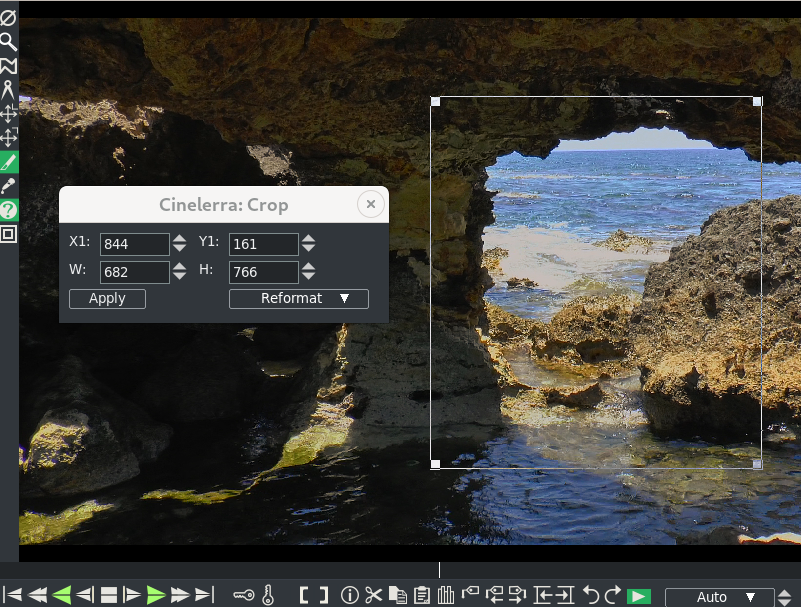
\includegraphics[width=0.5\linewidth]{images/cropped_area.png}
    \caption{Cropped area is in the top right corner}
    \label{fig:cropped_area}
\end{figure}

\begin{itemize}
    \item Enable the crop toggle and the tool window in the compositor window to display the Crop control dialog box.
    \item Click-drag anywhere in the video to define the crop area. This draws a rectangle over the video.
    \item Click-drag anywhere in the video to start a new rectangle.
    \item Click-drag over any corner of the rectangle to reposition the corner.
    \item Alt-click in the cropping rectangle to translate the rectangle to any position without resizing it.
    \item The crop control dialog allows text entry of the top left coordinates (X1,Y1) and bottom right coordinates (X2,Y2) that define the crop rectangle. When the rectangle is positioned, hit the \emph{Do it} button in the crop control dialog to execute the cropping operation: the portion of the image outside  the rectangle will be cut off and the projector will make the output fit the canvas.
    \item The Set Format window will show the new project Width and Height values.
    \item The projector tool window will show the new X, Y values.
    \item Track size will remain unchanged.
\end{itemize}
 
To undo the cropping enter the original project dimensions in the Set Format window and click on Reset projector in the popup menu of the compositor.

\subsection{Safe Regions}%
\label{sub:safe_regions}

On consumer displays the borders of the image are cut off and within the cut-off point is a region which is not always square like it is in the compositor window. 
The borders are intended for scratch room and vertical blanking data. 
You can show where these borders are by enabling the safe regions toggle. 
Keep titles inside the inner rectangle and keep action inside the outer rectangle.

\begin{figure}[htpb]
    \centering
    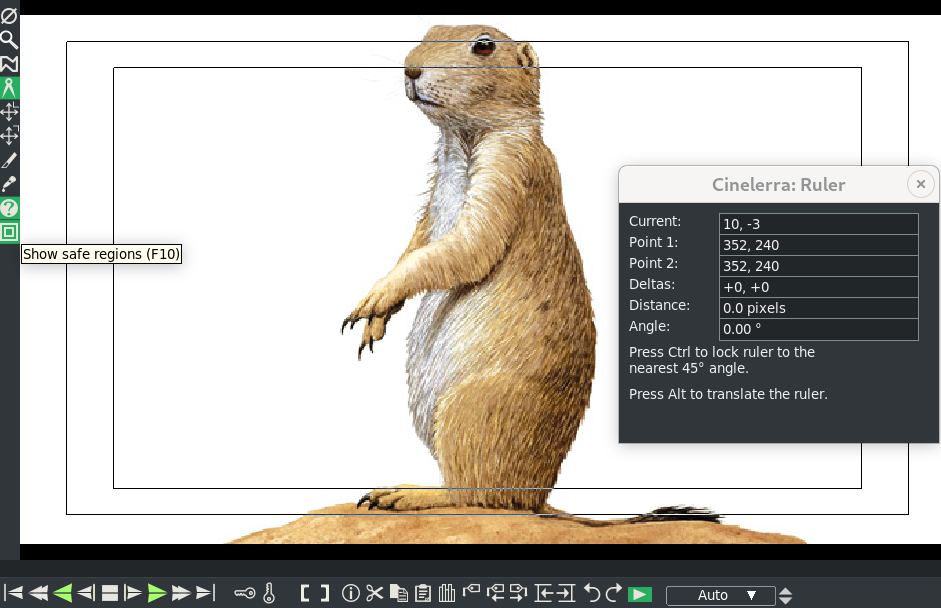
\includegraphics[width=0.6\linewidth]{images/safe_regions.png}
    \caption{Note the black frames showing the safe regions}
    \label{fig:safe_regions}
\end{figure}

\subsection{Track and Output Sizes}%
\label{sub:track_and_output_sizes}


The size of the temporary and the size of the output in our compositing pipeline are independent and variable. 
The camera's viewport is the temporary size. 
Effects are processed in the temporary and are affected by the temporary size. 
Projectors are rendered to the output and are affected by the output size. 
If the temporary is smaller than the output, the temporary is bordered by blank regions in the output. 
If the temporary is bigger than the output, the temporary is cropped.

\subsubsection*{Track size}%
\label{ssub:track_size}

The temporary size is defined as the track size. 
Each track has a different size. 
Right click on a track to bring up the track's menu. 
Select \emph{Resize Track} to resize the track to any arbitrary size. 
Alternatively you can select \emph{Match output size} to make the track the same size as the output. 
If you resize a track, then its appearance on the compositor changes accordingly. 
Using the relationship between the track and the project's output size you can effectively reduce or magnify the size of a particular track with regards to the final output and therefore create visual effects like split screens, pans, and zooms on the compositor.

\subsubsection*{Output size}%
\label{ssub:output_size}


The output size is set in either File$\rightarrow$\emph{New} when creating a new project or Settings $\rightarrow$ \emph{Format}. 
In the Resources window there is another way to change the output size. 
Right click on a video asset and select \emph{Match project size} to conform the output to the asset. 
When new tracks are created, the track size always conforms to the output size specified by these methods.

When rendering, the project's output size is the final video track size where the temporary pipeline is rendered into.  
If the output size is larger than the temporary then the image transferred from the temporary will fit inside the Output Track. 
Any space left on the Output is left blank.  
If the output size is smaller than the temporary then some of the temporary video will be cropped.

\section{Viewer Window}%
\label{sec:viewer_window}

The viewer window (figure~\ref{fig:viewer_window}) is a place to load and preview your source media and clips.  
Here you can quickly browse through an asset using the slider control, focus on an area of work with the preview region or you use editing controls to cut and paste segments into the project or create a clip for later use.

\begin{figure}[htpb]
    \centering
    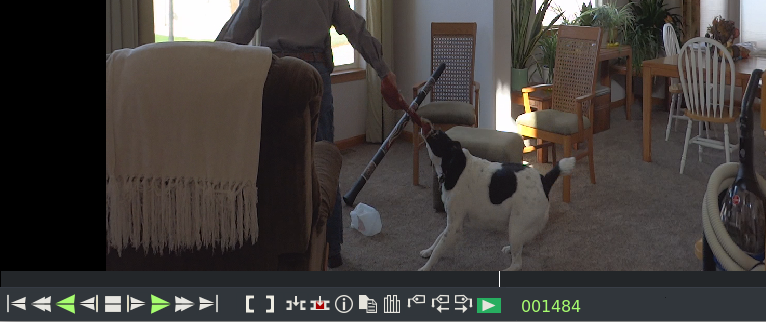
\includegraphics[width=0.99\linewidth]{images/viewer_window.png}
    \caption{Viewer Window}
    \label{fig:viewer_window}
\end{figure}

To open the viewer window, go to Window$\rightarrow$Show Viewer.  
The display is the area on the viewer where you actually see media playing.  
Before you can play any media, you must first load it on the viewer. 
To load media into the viewer:

\begin{enumerate}
    \item  Open the resources manager window and select the Media folder or the Clip folder.
    \item  Drag a file from the Media or the Clip folder to the viewer.
\end{enumerate}

You can also load media onto the viewer by right clicking on a file in the asset manager and selecting View from the popup menu or by double clicking on the icon. 
Once your media loads you will see it appear on the display. 
To play, rewind or forward through it use the slider control or the transport controls. 
You can change the media display size by right clicking on the screen to activate the display zoom menu. 
Select zoom levels of 50\%, 100\% or 200\% of the original media size.

When displaying media, the viewer uses the project's defined output size format settings, not the original assets format. 
You can change the project's output to match the asset's format using the match project size menu option in the asset manager. 
In the Viewer you can move around in the source media or clips and select regions to paste into the project. 
Operations done in the viewer affect a temporary EDL or a clip, but not the timeline.

\section{Options in both the Compositor and Viewer Windows}%
\label{sec:options_in_both_the_compositor_and_viewer_windows}

The next sections describe capabilities that are available in both the Compositor and Viewer windows.

\subsection{Click to Play in Viewer and Compositor}%
\label{sub:click_to_play_in_viewer_and_compositor}

In both the Viewer and Compositor windows, there is an arrow on the right hand side of the other buttons in the edit panel.  
Mouse action can be toggled on/off via this arrow, which has a tooltip of “Click to play” with the letter ‘p’ to be used for a shortcut.  
When enabled there is a gold-colored shadow around the usual green-colored arrow.  
The purpose of enabling this capability is to make it really easy to play the media in the window by just using the left mouse button to start or stop the play.  
The entire main canvas surface becomes a big play button!  
Although the default is initially off, a good reason to enable this, at least temporarily, is so that you can quickly review your video before a render. 
 
\begin{description}
    \item[left click]          forward play or stop forward play if already playing
    \item[middle wheel]  single frame forward or back
    \item[middle click]    reverse play or stop reverse play if already playing. 
        Note that some 3 button mice do not accommodate a middle click for reverse but you can find out by testing from a terminal window with the command xev.
\end{description}

\subsection{Timebar + Preview Region Usage in the Compositor and Viewer}%
\label{sub:timebar_preview_region_usage_in_the_compositor_and_viewer}

The navigation features of the Viewer and Compositor behave very similarly. 
Each has a timebar and slider below the video output. 
The timebar represents the entire time covered by the program.   
When you have a file loaded in the main window and then slide around it using the compositor slider. The insertion point in the main window follows the compositor. 

Labels and in/out points are fully supported in the viewer and compositor.  
In the viewer and compositor, labels and in/out points are displayed in the timebar.  
But there is a difference between the viewer and compositor in that the compositor reflects the state of the program while the viewer reflects the state of a clip but not the program. 
When you hit the label button in the compositor, the label appears both in the compositor timebar and the program timebar. 
When you select a label or in/out point in the compositor, the insertion point in the program window jumps to that position. 

The timebar in the compositor and the viewer can be used to define a region known as the preview region.  
This preview region is the region of the timeline which the slider affects.  
By using a preview region inside the entire program and using the slider inside the preview region you can very precisely and relatively quickly seek in the compositor and viewer.  
The preview region can be especially handy when you have large pieces of media by previewing one section, then move to the next section.  

The active preview region is the zone between the edge bars.  
The full range of the window slider pointer action is down-scaled to the active preview region.   
To use this, set the preview active region as a media time region of interest.  
Now addressing the timebar with the mouse only operates as if the timebar is zoomed to the scale of the active preview zone.  
This has the effect of magnifying the interesting media in terms of the mouse pointer addressing, for fine-tuning.

\begin{figure}[htpb]
    \centering
    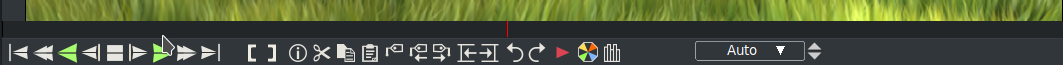
\includegraphics[width=0.8\linewidth]{images/timebar1.png}
    \caption{The arrow above the green colored “play forward” transport button is on the timebar.}
    \label{fig:timebar1}
\end{figure}

To create and use a preview region, hold down the right mouse button inside the timebar on either end of the timebar close to the edge until you see the resize pointer.  
While continuously holding the right mouse button down, drag the arrow away from the end towards the middle of the timebar until you have the desired area outlined.  
The slider will be a light blue color while the selected preview region will remain the same initial black color.  
There are either a left or right resize pointer and you can click and drag in either direction to expand or shrink the region.

\begin{figure}[htpb]
    \centering
    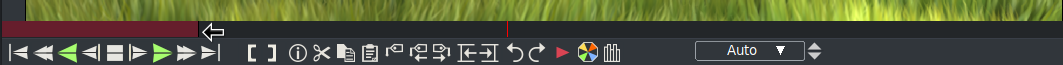
\includegraphics[width=0.8\linewidth]{images/timebar2.png}
    \caption{ A left-facing arrow on the right side of the blue slider bar is used to drag the bar.}
    \label{fig:timebar2}
\end{figure}

\begin{figure}[htpb]
    \centering
    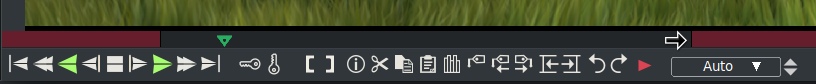
\includegraphics[width=0.8\linewidth]{images/timebar3.png}
    \caption{Here you can see the right-facing arrow used to drag the other end of the slider bar.  
        The black area between is the actual preview area.}
    \label{fig:timebar3}
\end{figure}

You can slide the preview zone left or right by holding the right mouse button over the preview zone where you will see a fat double headed arrow.  
The selected area will move left or right as you drag and still retains the same size.

\begin{figure}[htpb]
    \centering
    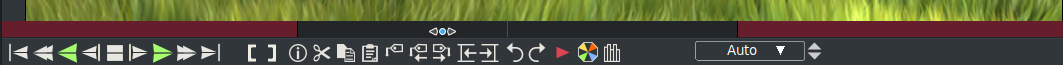
\includegraphics[width=0.8\linewidth]{images/timebar4.png}
    \caption{Note the double-headed fat arrow in the preview area used  to move the selection over.}
    \label{fig:timebar4}
\end{figure}

Settings:

\begin{enumerate}
    \item  If no preview region is set, increasing the length of the media on the timeline by inserting media or
        appending, has no effect on the non-selected preview region.  That is, you will not see the blue slider
        suddenly mysteriously appear.
    \item  If the preview region is set, when you replace the current project or file,  the preview region is
        automatically disabled.
    \item  If the preview region is set, when you append data or change the size of the current project, the
        preview region may appear to either move, shrink, or grow depending on the new length of the
        media on the timeline.  
    \item  To disable the preview region, you will have to drag both the right and the left blue slider bars
        completely to their corresponding end so that there is no longer any visible blue slider.
\end{enumerate}

A good method for taking advantage of the preview region is described here.  
On the main track canvas, scroll to the beginning of the area of interest.  
When you do that, you will see in the compositor the red indicator line of that location.  
Now in the compositor window, right mouse drag from the left side of the edge of the timebar to create the blue slider bar line up to the red indicator.  
Back in the main track canvas, move to the location of the area you want to end looking and again you will see the red indicator line in the compositor.  
Use the right mouse drag from the right to stop at that end point.  Using this method is often easier than continuous usage of the single frame move which can be tedious.

One last interesting item of note --- sometimes you may wish to see just a little more that is outside the preview region and you can do so!  You can actually move outside the compositor or viewer window space and view more, at least until you hit the end of the monitor space.

\section{Resources Window}%
\label{sec:resources_window}

Effects, transitions, labels, clips, proxies, user bins, and media assets are accessed here. 
Most of the resources are inserted into the project by dragging them out of the resource window. 
Management of resource allocation is also performed here.

\begin{figure}[htpb]
    \centering
    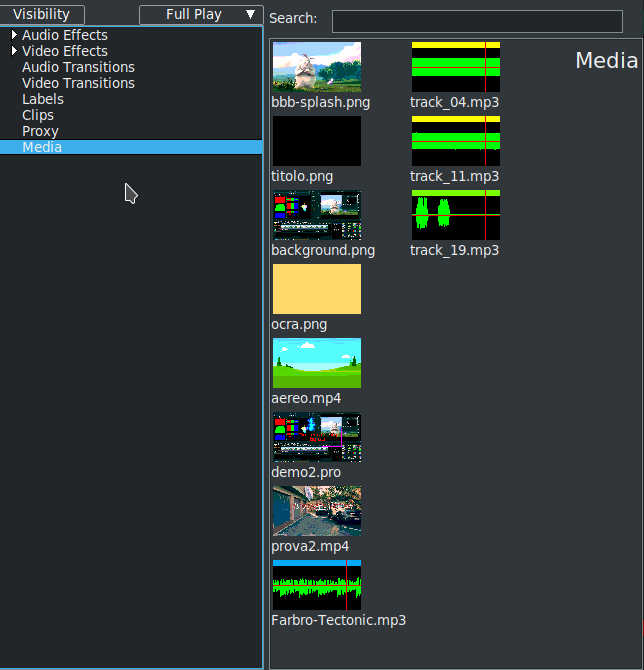
\includegraphics[width=0.99\linewidth]{images/resource_window.png}
    \caption{Folders are in the first column with contents of that folder on the right hand side}
    \label{fig:resource_window}
\end{figure}

The resources window is divided into two areas (figure~\ref{fig:resource_window}. 
One area lists folders and another area lists the folder contents. 
Going into the folder list and clicking on a folder updates the contents area with the contents of that folder. 
The folders can be displayed as icons or text. 
There are several variations for displaying the contents; select \emph{Display text}, \emph{Display icons}, \emph{Display icons packed}, \emph{Display icons list} as types of display for the assets or plugins. 
Use the letter “v” to easily scroll through the choices and see which you prefer.  
You can also get to these options from the menu by a right mouse click in the window.

A \emph{Search} option is available for any of the folders in the Resources window (and when using “Attach effect” on the main track canvas for the Plugins).  
As you type in characters a match is made with that substring.  
Names that do not match are filtered out making it a lot easier to find the item you are looking for.  
The characters can be any where within the phrase and it does not matter if upper or lower case. 

Other options you will see if you \textbf{right mouse click in the folder} which brings up the menu are described next.  

\begin{description}
    \item[ Load files ]  for convenience to load files same as from the main window so you do not have to move the mouse so far in case you have multiple monitors.
    \item[Display text/icons]  as described previously for format variations preference.
    \item[Select]  options are All, Used, Unused, and None.  This gives you the capability to have a set of the
        contents highlighted for ease of use so you can see what is or is not loaded, or unset the highlight.
    \item[Sort items]  to sort the contents of the folder alphabetically.  Especially helpful if you accidentally did a 
        drag and changed your mind or dropped suddenly so that the assets no longer look nicely aligned.
    \item[Copy/Paste file list]  use to easily copy a set of files or paste a set of files between Cin and windows.
    \item[Snapshot/Grabshot]  described elsewhere in more detail.
\end{description}

Using the right mouse click to bring up a menu in the folder area, you can also switch from Display text to Display icons, Sort items and create, delete and manipulate user defined folders/bins. Select Folder to create a user Folder or modify an existing folder.

If you \textbf{right mouse click on a highlighted/selected resource}, several options are available depending on whether the resource is an effect or transition or a piece of media.  
You can highlight several for some options so that it is applicable to all of them, such as Info.  
Those listed immediately below are the available choices for media assets.


\begin{description}
    \item[Info]  provided basic Asset information; details are described later in this section.
    \item[Display text/icons]  same as mentioned previously.
    \item[Sort]  same as mentioned previously.
    \item[Rebuild index] if you switch from/to using ffmpeg/native for media loading, you should rebuild
        indexes.  Or if you get hangs on media or strange looking tracks, you might want to rebuild indexes.
    \item[View]  use this option to bring up the media in the Viewer window.
    \item[View in new window]  in order to not overwrite your current viewer window, you can open any
        number of viewer windows to simultaneously view multiple media.
    \item[Open mixers]  when you record with multiple cameras setup, you can work with them most easily
        using the mixer mode.  This is described in detail
    \item[Paste]  
    \item[Match]  if you need to change your media parameters you can choose from the following: Match frame
        rate, Match project size, Match all 
    \item[Remove]  use to Remove the asset from the project or with caution, to Remove from disk permanently.
\end{description}

In the case of Effects or Transitions, a right mouse click on a highlighted selection leads to an \emph{Info} button which gives a short 1 line description of what the effect/transition can be used for.
For Labels, choices are \emph{Edit}, \emph{Label}, and \emph{Go to}.
For Clips, \emph{Nest} and \emph{UnNest} as described elsewhere are available.

\subsection{Info Asset Details}%
\label{sub:info_asset_details}

The asset \emph{Info} window also can be used to display detailed information about the selected/highlighted media file --- available for any loaded media of type mpeg or ffmpeg.  
This is extremely helpful in determining what type of media it is, size, resolution, format, and type/number of audio streams.  It is especially useful for multiple program streams.  You can have the info window popped on several of your assets simultaneously.

Figure~\ref{fig:info_asset_details} shows the “Detail” box to click on the left side and a simple, typical output in the Asset Detail window on the right side.  Also, note the highlighted media in the Resources window.

\begin{figure}[htpb]
    \centering
    \includegraphics[width=0.99\linewidth]{images/info_asset_details.png}
    \caption{The “Detail” box}
    \label{fig:info_asset_details}
\end{figure}

\subsection{User Folders/Bins}%
\label{sub:user_folders_bins}

Creating folders that are more specific to a particular project is helpful in better organizing your work.  
This can be done by utilizing the files already loaded to the “master” Media or Clips folders in the Resources window.  
Below are steps illustrating an easy way to set up a folder.

%TODO Below part need to be rewriten
\begin{enumerate}
    \item In the Resources window (figure~\ref{fig:folder_resources}), in the location of the Video/Audio effects and Media folders, bring up the “Folder...” popup by clicking the right mouse button.  
        Highlight, then click “New Media or Clips”.
        \begin{figure}[htpb]
            \begin{minipage}{.55\linewidth}
                \centering
                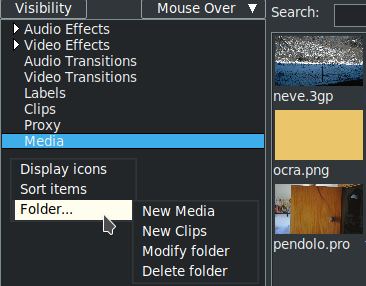
\includegraphics[width=0.9\linewidth]{images/folder_resources.png}
                \caption{Highlight, then click “New Media or Clips”.
                    “Modify folder” can be used to   change the name of a folder.
                    “Delete folder” in the popup can be used to delete a folder.
                }
                \label{fig:folder_resources}
            \end{minipage}
            \hfill
            \begin{minipage}{.35\linewidth}
                \centering
                \vspace{18ex}

                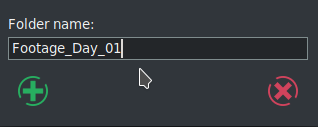
\includegraphics[width=0.9\linewidth]{images/folder_new.png}
                \caption{Type in your folder name in the textbox.  Click OK.}
                \label{fig:folder_new}
            \end{minipage}
        \end{figure}
    \item  In the “New folder” popup as shown below (figure~\ref{fig:folder_new}), type in your folder name in the textbox.  Click OK.
        \begin{figure}[htpb]
            \centering
        \end{figure}
    \item  Select the “master” Media folder to see which files are currently loaded, figure~\ref{fig:folder_master}.  
        Highlight the files there that you want to copy to your new folder (named Photos of Garden).  
        Drag the files to the left and when you see the Photos of Garden folder become highlighted, then drop there.  
        You can drag and drop any of the media from the “master” Media at any time.  
        It flashes when the drop is successful.
\end{enumerate}

\begin{wrapfigure}[12]{O}{0.53\linewidth} 
    %\vspace{-2ex}
    \centering
    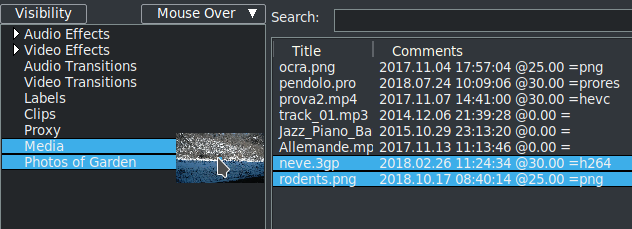
\includegraphics[width=0.9\linewidth]{images/folder_master.png}
    \caption{The “master” Media folder}
    \label{fig:folder_master}
\end{wrapfigure}

Adding the Shift key before the actual drop, will allow for relative path filenames instead of full path.
But you might want to include or eliminate some of the media that exists in one of the folders that you have set up already.  
In this case you will want to click on the “Modify folder” in the popup.  
When you bring up the Modify folder window, if you already have files in that folder, you will see filters that were generated automatically when you did a Drag and Drop.


\begin{figure}[htpb]
    \centering
    %\includegraphics[width=0.8\linewidth]{name.ext}
    \begin{tikzpicture}[scale=1, transform shape]
        \node (img1) [yshift=0cm, xshift=0cm, rotate=0] {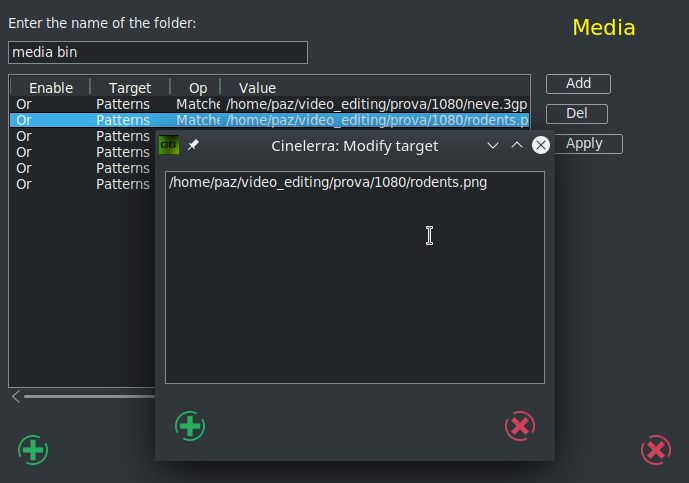
\includegraphics[width=0.7\linewidth]{images/folder_modify.png}};
        \node [yshift=-29mm, xshift=-1cm,anchor=east] at (img1.north west) (Arrow1) {\parbox{8em}{Here is the filter that was generated with the original drop }};
        \node [yshift=-85mm, xshift=0cm,anchor=east] at (img1.north west) (Arrow2) {\parbox{10em}{When you click on the Value portion of that filter, the entire set of files that are covered by the filter rules pops up.   Now you can highlight a target filename that you would like to remove, and just erase that line and check the green checkmark for OK.}};
        \draw [->, line width=1mm] (Arrow1) edge  ([yshift=-29mm] img1.north west);
        \end{tikzpicture}
    
    \caption{Modify target}
    \label{fig:modify-target}
\end{figure}

To delete the entire set of files listed on the filter rule, highlight the rule line and hit the “Del” button.  
To add a new filter rule, click on the “Add” button which will automatically add a default line after any current lines.  
The default line will be a line that matches everything in the “master” Media folder which is “Or  Patterns  Matches   *”.  
Click the right mouse button on the current field underneath the column header to see the choices available for each column.  

Modifications will not be in effect until you click on the green arrow OK button or click on the Apply button.  
But once you hit Apply, clicking on the red X button will not undo your changes.  
The filter/search rules are applied in the order listed in the Modify folder window.  
You can change the order of the filter rules by highlighting the rule you want to move and then drag and drop to a new location.

The figure~\ref{fig:modify_folder} below displays the available choices for each field.

\begin{figure}[htpb]
    \centering
    %\includegraphics[width=0.8\linewidth]{name.ext}
    \begin{tikzpicture}[scale=1, transform shape]
        \node (img1) [yshift=0cm, xshift=0cm, rotate=0] {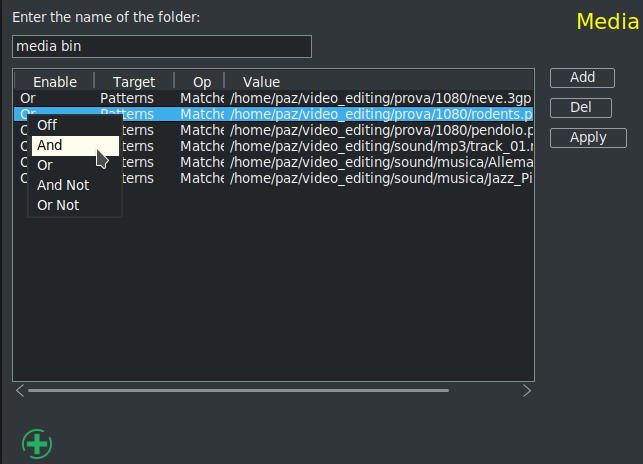
\includegraphics[width=0.6\linewidth]{images/modify_folder1.png}};
        \node (img2) [yshift=-1cm, xshift=4cm, rotate=0] at (img1) {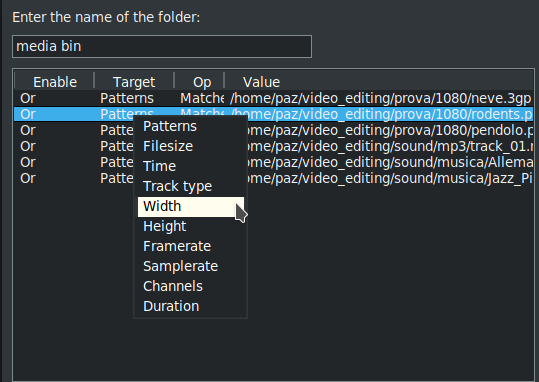
\includegraphics[width=0.6\linewidth]{images/modify_folder2.png}};
        \node (img3) [yshift=-1cm, xshift=3cm, rotate=0] at (img2){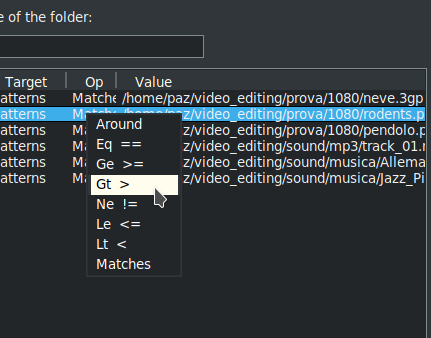
\includegraphics[width=0.3\linewidth]{images/modify_folder3.png}};
    \end{tikzpicture}
    \caption{The available choices for each field}
    \label{fig:modify_folder}
\end{figure}

Information about the columns and rules for the search filters in the Modify folder window follows.

Column headers:

\begin{description}
\item[ Enable]  this column is used to designate the state of that filter rule
    \begin{description}
        \item[ Off]		disable the filter
                \item[And] 		narrow your search; all of your search terms must be present
                \item[Or]		broaden your search to include more values
                \item[And Not]	exclude terms that do not contain the given value from your search results
                \item[Or Not]	include terms that do not contain the given value from your search results
    \end{description}
\item [Target] – this column designates which media asset attribute to look at
    \begin{description}
        \item[ Patterns]	each line contains a filename filter, matches the file path
                \item[Filesize]	number of bytes in a file
                \item[Time]		date file was created
                \item[Track Type]	track type of video, audio, or audio video (for both)
                \item[Width]	Format width
                \item[Height]	Format height
                \item[Framerate]	Video framerate
                \item[Samplerate]	Audio samplerate
                \item[Channels]	Number of audio channels
                \item[Duration]	Playback time in seconds --- it uses the largest of audio or video if contains both
    \end{description}
\item[Op] – boolean operators used to narrow or broaden the relationship between your search terms
    \begin{description}
        \item[Around]	about this value; use “+radius” for a search range: [target–radius ...  target+radius]
        \item[Eq	]	equal to
        \item[Ge]	greater than or equal to
        \item[Gt]	greater than
        \item[Ne]not equal
        \item[Le]	less than or equal
        \item[Lt] less than
        \item[Matches]	exactly matches for strings
    \end{description}
\end{description}

\textbf{Value} --- the characteristic you are looking for with expressions that can be written with the following:

\begin{description}
\item[Number] (decimal points are allowed and will be converted to a standard form):
    \begin{description}
        \item[inf] representing infinity
        \item[\#[TtGgMmKk]]  ---  where \# represents a number and the characters mean:
    \end{description}

    \begin{tabular}{rcl}
        inf&=& infinity\\
        T&=&1099511627776\\
        t&=&1000000000000\\
        G&=&1073741824\\
        g&=&1000000000\\
        M&=&1048576\\
        m&=&1000000\\
        K&=&1024\\
        k&=&1000\\
    \end{tabular}

\item[Scalar:] 

    \begin{tabular}{l}
        Number\\
        Number+Number\\
    \end{tabular}
\item[Date time:]
    \begin{tabular}{rcl}
        date&=&year/month\\
        date&=&year/month/day\\
        time&=&hour:minute\\
        time&=&hour:minute:second\\
        date\_time&=&date time\\
    \end{tabular}

  \item[Duration:]
      \begin{tabular}{rcl}
    day  &=&	\#day 	  | \#days\\
    week &=&	\#week 	  | \#weeks\\
    month&=&	\#month | \#months\\
    year &=&	\#year	  | \#years\\
    delta&=&secs\\
    delta&=&mins:secs\\
    delta&=&hours:mins:secs\\
      \end{tabular}

\item[Around time:]
    date time+duration

  \item[Around length:]
    duration+duration

\end{description}

Table showing the allowed usage:

%TODO create table for below code
\begin{lstlisting}[numbers=none]
target:    |  eq  ge  gt  ne  le  lt   matches  around
++++++++++++++++++++++++++++++++++++++++++++++++++++++++
patterns   | <---- strcmp ---------> + filter + nearest
file_size  | <---- arithmetic -------+------> + radius
mod_time   | <---- arithmetic -------+------> + radius
track_type | <---- member test ------+--------+------>
width      | <---- arithmetic -------+------> + radius
height     | <---- arithmetic -------+------> + radius
framerate  | <---- arithmetic -------+------> + radius
samplerate | <---- arithmetic -------+------> + radius
channels   | <---- arithmetic -------+------> + radius
duration   | <---- arithmetic -------+------> + radius
\end{lstlisting}

where in the above, the filter can be:

\begin{tabular}{rcl}
    filter&=&list\\
    filter&=&token\\
    list&=&[token]\\
    list&=&[token]list\\
    string&=&<chars>|<empty>\\
    token&=&string\\
    token&=&string*token\\
\end{tabular}

Examples with some caveats first:

\begin{enumerate}
    \item   “Or” generally includes or adds whereas “And” generally excludes or subtracts.
    \item   The filters only work on media in the folder; if there is no media, then there is nothing to search.
    \item   The examples below are not meant to be executed as a list of filters in Modify folder, they are just single line examples to indicate what can work.
    \item   Sort is by filename base name (directory path not included automatically) except when the “Around” operation is used and then it is sorted by that Target distance first and then filename.
\end{enumerate}

\begin{table}[htpb]
    \centering
    \caption{Examples}
    \label{tab:label}
    \small
    \begin{tabular}{llllm{10em}} \toprule
        Enable&	Target&	Op&	Value&	meaning\\\midrule
Or	&Patterns  &Matches   &*&	 all files from the Media folder are included\\
And Not&Filesize&Lt	&160000000& no files that are less than 160MB in size \\
Or Not&	Time	&Ge	&2018/07/30 06:13:00	& files not greater than or equal date\\
And	&Duration&Eq	&01:00		& files included must have 60 secs. Duration\\
Off	&Samplerate&Ne	&44000		& off for now, but may want to include later\\
And	&Framerate&Around&24+1		& files included all have 24 to 25 framerate\\
Or	&Patterns&Matches&[*.mp4]	& all files with the extension of mp4\\
Or	&Time&	Around&2018/08/02 06:00:00 + 02:00:00  & files at 4AM to 8 AM\\\bottomrule
    \end{tabular}
\end{table}


\subsection{Vicons \& Aicons – aka Video Icons / Audio Icons}%
\label{sub:vicons_aicons_aka_video_icons_audio_icons}

Vicons are video icons.  
Aicons are audio icons.  
By default the Resources window will play the first 5 seconds of video or audio waveform looped in the area occupied by the media icons (figure~\ref{fig:vicons1}). 
This is enabled for the Media/Proxy folders in icon mode when the mouse pointer is inside the Resources window. 

\begin{figure}[htpb]
    \centering
    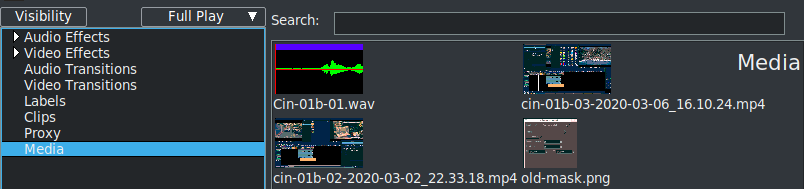
\includegraphics[width=0.99\linewidth]{images/vicons1.png}
    \caption{Note "Full Play" mode and Vicons and Aicons in Media folder}
    \label{fig:vicons1}
\end{figure}

The waveform in the figure~\ref{fig:vicons2} is displayed in the Resources window in the color green/yellow for the 2 audio tracks. 
There is a colored bar on the top of each a-icon where the color is based on the Color Spectrum --- the smaller the time duration, the redder the color; then as the time duration goes up, the color goes up so that you will go to green, then yellow, then blue, then really dark blue, then purple for the audio files 1 hour and over.  
There are various other colors between these colors same as that seen in the color spectrum in the screenshot below.  
Colors are utilized from the hue wheel in the counter-clockwise direction.  
Note that the horizontal line in the middle of the a-icon is yellow/red representing the 2 audio tracks and is only red for mono.



\begin{figure}[htpb]
    \centering
    %\includegraphics[width=0.8\linewidth]{name.ext}
    \begin{tikzpicture}[scale=1, transform shape]
        \node (img1) [yshift=0cm, xshift=0cm, rotate=0] {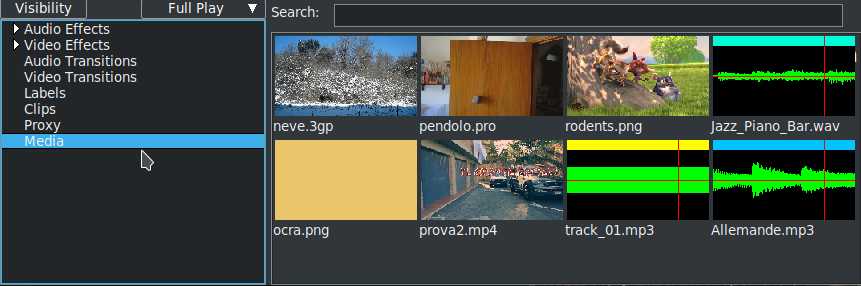
\includegraphics[width=0.99\linewidth]{images/vicons2.png}};
        \node (img2) [yshift=0cm, xshift=2.8cm, rotate=0] at (img1.south west) {\includegraphics[width=0.3\linewidth]{images/hue_wheel.png}};
        \node [yshift=-5mm, xshift=1cm,anchor=west] at (img2.east) (Arrow1) {\parbox{18em}{Color hue wheel. For illustration only}};
        \draw [->, line width=1mm] (Arrow1) edge  ([yshift=-5mm] img2.east);
    \end{tikzpicture}
    \caption{Draw Vicons   |            Screenshot display various audio file lengths; red is shortest.}
    \label{fig:vicons2}
\end{figure}

Note that if in Settings$\rightarrow$Preferences under the Appearance tab, you have unchecked “Use thumbnails in resource window” you will only have default icons and none of the above capabilities.


\subsection{Resources Window Preview Mode}%
\label{sub:resources_window_preview_mode}


Preview mode can be used to pop up a window which draws the vicons/aicons thumbnails in a larger size.  
Preview or “draw vicons” mode is a helpful feature of cinelerra that lets you see and/or hear the first 5 seconds of the video for identification purposes. 
The Preview mode/playback toggle is to the right of the Visibility label as seen in the screenshot above. 
Preview mode is available for the Media, Proxy, Media User Bins, and Clips but clips are only 1 image.

When “Preview”/“draw vicons” is enabled/active, if you click on one of the video icons or an audio waveform icon, a view pops up that increases the size to 4 times the surface area larger. 
This makes it easier to see or hear if it is the media you are looking for in case you have many similar media files. 
To conserve memory, the video is stored 8-bits per pixel which results in low image quality while the audio is 16-bit. 
The reason for playing 5 seconds of a video for a vicon is that until the first I-frame, the media frequently does not decode properly.  
In other words, a lot of media does not begin at the “beginning” point and will not be properly rendered until enough data has been read to assemble a picture.  
You can increase the thumbnail size, clarity of pixels (memory size) and color mode but it takes a lot more memory.  
Change these values in Settings$\rightarrow$Preferences, Appearance tab, right hand side of the Layout section – be aware that when you click OK, your session will re-initialize.  
You can also temporarily increase the preview mini-window by use of the mouse wheel up or down.

There are 4 options for the preview mode.

\begin{enumerate}
    \item  \emph{Full Play} is the default mode.  
        This means all of the media will automatically play when the mouse is in the Resources window and you can use the left mouse button to click on specific media to see it pop up in a larger view.  
        Audio only files do not play the audio until the icon is clicked on and the waveform aicon pops up into the 4x larger mode. 
        \emph{Full Play} includes the \emph{Mouse Over} capabilities as described below as well as the Inter-View \emph{Src Target} functions.

\item  \emph{No Play} mode is especially useful on smaller computers and for users who find the constant loop play to be somewhat distracting.

\item  \emph{Mouse Over} mode is activated by a single click on one of the vicons/aicons and deactivated with another single click over any of the icons.  
    Once activated, whenever you just move the mouse over an icon, it automatically pops up the increased size preview.  
    The first time in your session that you enable this feature, it may take a few seconds to load all of the icon previews into memory so be patient and just wait.  
    \emph{Mouse Over} mode makes it quick and easy to preview without having to drag the media to the viewer.  
    You can still drag the media same as without preview enabled.  

\item  \emph{Src Target} mode gives easy access to the Inter-View source target available by using the middle mouse button on media.  
    There are 2 advantages to this mode --- there is no 5 second play loop taking up cpu time and the popup allows for the use of the letter “f” on that popup to have it go to fullscreen mode.  
    \emph{Src Target} mode in any scenario never plays sound as that is nonsensical usage.  
    After the initial click to pop media in this mode, you also have the \emph{Mouse over} feature.
\end{enumerate}

For any of the options, but not \emph{No Play}, you can temporarily turn off that option by clicking on the button using the middle mouse button.  
This helps to avoid having the thumbnail get in the way of dragging or other functions.  
When you do, a line will be drawn through the current preview mode so that you are aware that it is in \emph{No Play} mode until click it again.

Note that if in Settings$\rightarrow$Preferences under the Appearance tab, you have unchecked “Use thumbnails in resource window” you will only have default icons and no active previews.

\begin{figure}[htpb]
    \begin{minipage}{.69\linewidth}
        \centering
        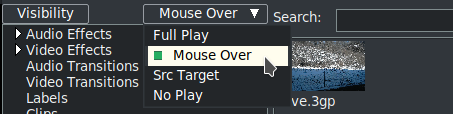
\includegraphics[width=0.99\linewidth]{images/preview_icon_mode.png}
        \caption{The location of the Preview/Draw Icons mode.}
        \label{fig:preview_icon_mode}
    \end{minipage}
    \hfill
    \begin{minipage}{.29\linewidth}
        \vspace{2ex}
        \centering
        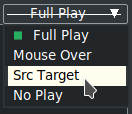
\includegraphics[width=0.7\linewidth]{images/line_through_mode.png}
        \caption{Note the line through the mode.}
        \label{fig:line_through_mode}
    \end{minipage}
\end{figure}



\subsection{Moving clips/media from/to Resources window}%
\label{sub:moving_clips_media_from_to_resources_window}

If you have several media files loaded into the Resources window of one instance of Cinelerra and want to load some of the same ones into another instance or just want a listing to save in a file for later use, you can do this with these set of steps:

Copy or paste a list of files in the Media Resources window:  


\begin{enumerate}
    \item  create a highlighted selection of the desired media files in the media Resources window
    \item    right click on an unused portion of that window to bring up the popup menu
    \item     select the “Copy file list” item and a file list box will appear that contains the full path filenames
    \item     wipe the textbox using your standard copy/paste method to put the list of files in the copy buffer
    \item     in another cinelerra instance, choose the “Paste file list” of the media Resources window
    \item     paste the list of files, again using your standard paste method, into the new file list box; press OK
    \item    the status bar of the main window will be updated as the file list is loaded to the media folder (the purpose of displaying the status is simply to show that the load is progressing normally).
\end{enumerate}

Obviously this “Paste file list” feature means you can create a list of files outside of cinelerra using an editor, wipe the names, and then use “Paste file list” to load them into the media Resources window.  

It is important to note that in the steps above, the Operating System cut and paste capabilities are in use for steps 4 and 6 as opposed to Cinelerra’s c/v shortcuts.  
Since the procedure varies among the distros, you will have to adapt to your specific one.  For example, a usage for ubuntu consists of:
\begin{enumerate}
    \setcounter{enumi}{3}
    \item   Ctrl-c to copy the list of files; open gedit; Ctrl-v to paste the list of files into gedit
    \item   Ctrl-c or the standard way using the right click to copy this list from gedit
    \item Ctrl-v paste the list of files into the new file list box, and press OK
\end{enumerate}

\begin{figure}[htpb]
    \centering
    \begin{minipage}{.49\linewidth}
    \centering
        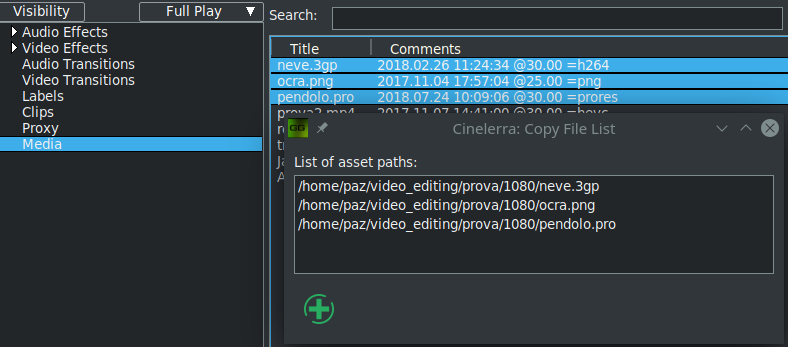
\includegraphics[width=0.99\linewidth]{images/copy_files1.png}
    \end{minipage}
    \hfill
    \begin{minipage}{.49\linewidth}
    \centering
        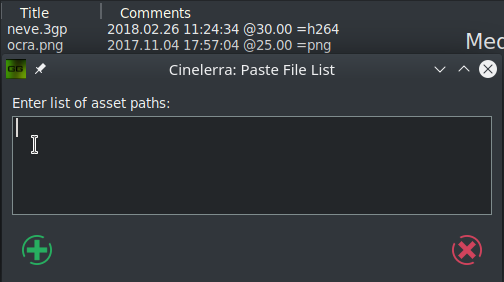
\includegraphics[width=0.99\linewidth]{images/copy_files2.png}
    \end{minipage}
    \caption{Example of copy file list}
    \label{fig:copy_files1}
\end{figure}

In the Figure~\ref{fig:copy_files1}, one instance of cinelerra has 6 items in the Media area highlighted that were copied to the file list.  
Note how it includes the full pathname.

In this screenshot on another instance of cinelerra, there are only 2 items in the media but the “Paste file list” box is ready to have the items inserted via the standard text box paste method.  When that is done, the additional 6 media files will be available on this other instance too.


Another possible usage of this capability:

\begin{enumerate}
    \item  Right Click on the Clips Resources window and use the “Paste Clip” option to paste the Copy selection as a clip.  
    \item  Similarly, by highlighting a clip in the Resources window and selecting its copy popup menu item using the right mouse button, that copy buffer can now be loaded onto the timeline.
\end{enumerate}


\subsection{Snapshot / Grabshot}%
\label{sub:snapshot_grabshot}

\begin{figure}[htpb]
    \centering
    \begin{minipage}{.49\linewidth}
    \centering
    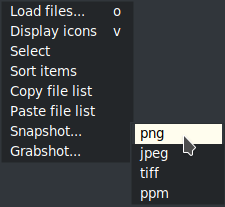
\includegraphics[width=0.8\linewidth]{images/snapshot.png}
    \caption{Snapshot menu and choices}
    \label{fig:snapshot}
    \end{minipage}
    \begin{minipage}{.49\linewidth}
    \centering
    \begin{tikzpicture}[scale=1, transform shape]
        \node (img1) [yshift=0cm, xshift=0cm, rotate=0] {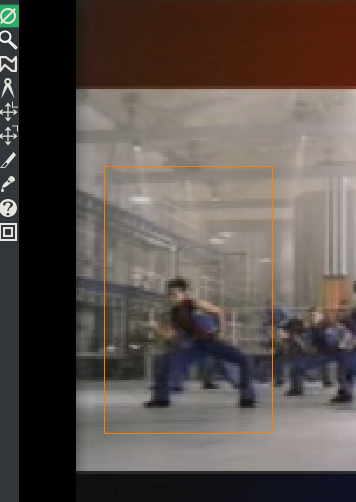
\includegraphics[width=0.65\linewidth]{images/grabshot.png}};
        \node (img2) [yshift=2cm, xshift=-1cm, rotate=0] {\includegraphics[width=0.07\linewidth]{images/reticle.png}};
    \end{tikzpicture}
    \caption{Grabshot reticle \& orange box}
    \label{fig:grabshot_recticle}
    \end{minipage}
\end{figure}

To take a snapshot, perform the following steps:

\begin{enumerate}
    \item set your timeline insert marker where you want the snapshot --- this frame shows in the compositor
    \item  right click in an empty spot in the media folder and the popup shows snapshot as the 5th item down
    \item  highlight that and the submenu comes up allowing you to choose png, jpg, ppm or tiff
\end{enumerate}

The snapshot shows up in the Media folder.  
It is saved by default in \texttt{/tmp} as \texttt{snap\_date-time.ext} BUT you can change the default directory path in Settings $\rightarrow$ Preferences $\rightarrow$Interface tab in the right hand side of the Editing section.

Grabshot is the 6\textsuperscript{th} menu item.  
A red circle reticle can be moved to the area to grab; use left mouse drag to surround an area; and right click to grab.




\section{Other Options and Other Windows}%
\label{sec:other_options_and_other_windows}

\subsection{Transport Controls}%
\label{sub:transport_controls}

Transport controls are useful for navigation and for playing media.  
Each of the Viewer, Compositor, and Program windows has its own transport panel.  
The controls generally all contain a yellow colored tooltip when you mouse over the control, providing a hint of their function and shortcuts for usage.

The transport panel is controlled by the keyboard as well as the graphical interface. 
For each of the operations it performs, the starting position is the position of the insertion point in the Program window and the slider in the Compositor and Viewer windows. 
The ending position is either the end or start of the timeline or the end or start of the selected region if there is one.

The orientation of the end or start depends on the direction of playback. 
If it is forward the end position is the end of the selected region. 
If it is backward the end position is the start of the selected region.  
The insertion point moves to track playback. 
When playback stops, the insertion point stays where playback stopped. 
Thus, by playing back you change the position of the insertion point. 
The keyboard interface of either the numeric pad or alternative keys has more speeds with the addition of \emph{Forward Slow}(2) and \emph{Reverse Slow} (5).  
Hitting any key on the keyboard twice pauses it. 
The shortcuts section of this manual as well as a Shell Command available from the Cinelerra main window has a listing of each of the keys.

When using frame advance functions the behavior may seem odd. 
If you frame advance forward and then frame advance backward, the displayed frame does not change. 
This is because the playback position is not the frame but the time between two frames. 
The rendered frame is the area that the playback position crosses. 
When you increment the time between two frames by one and decrement it by one, you cross the same frame both times and so the same frame is displayed.  
There is an option in Settings$\rightarrow$Preferences, Appearance tab to “Always show next frame” that may help make this clearer for some users.

The transport behavior changes if you hold down Ctrl when issuing any of the transport commands. This causes the starting point to be the In point if playing forward and the Out point if playing backward. If playing forward, the Out point becomes the ending point and if playing backward, the In point becomes the ending point. If no In/Out points are specified, the behavior falls back to using the insertion point and track boundaries as the starting and ending points.

The transport behavior also changes if you hold down the Shift key along with KeyPad 1--6.  
If normally audio is included in the play, it will be removed and if normally audio is not included in the play, it will be added.


\subsection{Zoombar}%
\label{sub:zoombar}

The compositor has zoom capability. 
The pull-down menu on the bottom of the compositor window has a number of zoom options. 
When set to Auto the video is zoomed to match the compositor window size as closely as possible. 
When set to any other percentage, the video is zoomed a power of 2 and scrollbars can be used to scroll around the output. 
When the video is zoomed bigger than the window size,  you can use scrollbars to scan around or if the zoom icon is enabled, the middle mouse button can be used to zoom in or out the video.

The zoom toggle also causes the Compositor window to enter zoom mode. 
In zoom mode, clicking in the video output zooms in while a Ctrl-click in the video output zooms out. 
If you have a wheel mouse, rotating the wheel zooms in or out too. 
Zooming in or out with the zoom tool does not change the rendered output. 
It is merely for scrutinizing video or fitting it in the desktop. Playing video on the compositor when zoomed to any size other that 100\%, the original size, requires Cinelerra to do extra processing steps. 
This could affect performance on slower systems

\subsection{Show Overlays}%
\label{sub:show_overlays}

Color Coded Keyframe Curves are a big feature in the “Show Overlays” window because by changing the colors to suit the user, it helps to remove confusion from multiple curves on the track canvas.  
They can be viewed from the pulldown menu of Window$\rightarrow$Show overlays but they will operate the same as when used from the View pulldown menu.  
The “Color Coded Keyframe Curves” have distinct colors associated with each type for ease of identification.  
By clicking button 1 on the “Color Ball” to the right of any keyframe type in the “Show overlays” menu you have the ability to change the colors to whatever works best for your video.  
The color ball changes made will be retained across sessions.

There is a line separating the first 4 items, which are just non-automation type settable values as opposed to “auto” keyframe types.  
The color is not changeable for the 3 items of Mode, Pan, and Mask which simply display their symbol icon.

Screenshot below displays the Show overlays popup with all of its options and color coded types such as yellow for Speed and blue for Camera Z.  
Upon clicking on the associated “color ball” to the right of any keyframe type, for example “Fade” in this screenshot, the color wheel palette window pops up so that you can manipulate the color as desired.

\begin{figure}[htpb]
    \centering
    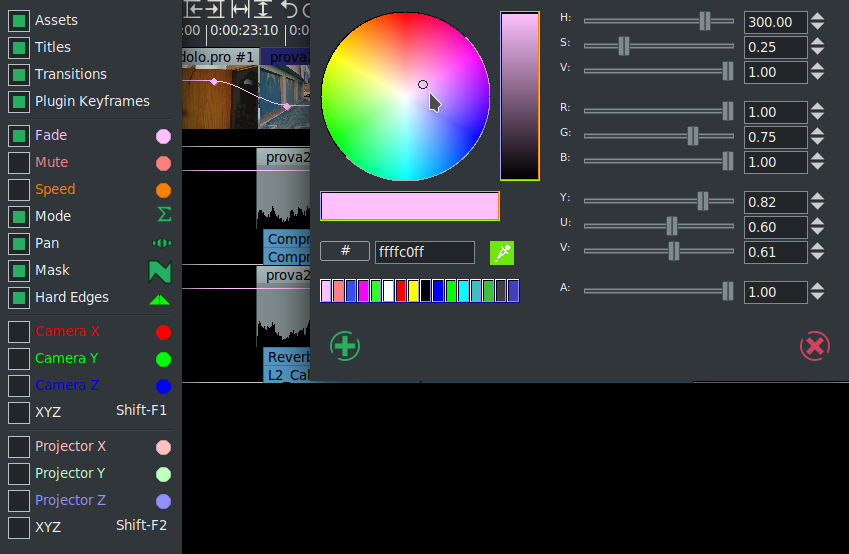
\includegraphics[width=0.99\linewidth]{images/overlays_window.png}
    \caption{Show Overlays window on the left with the Color ball window to the right to set color}
    \label{fig:overlays_window}
\end{figure}

Screenshot below shows several color coded lines for different keyframes along with the Fade slider for manipulation.  
The slider is in the same color as the color coded keyframe type line which is the same color as in the “Show overlays” window.

\begin{figure}[htpb]
    \centering
    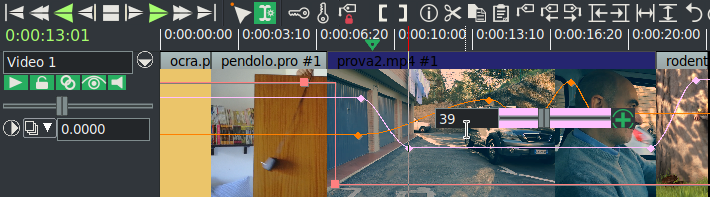
\includegraphics[width=0.8\linewidth]{images/overlays1.png}
    \caption{Lines are colored here on the timeline as designated in Show Overlays}
    \label{fig:overlays1}
\end{figure}

Overlays Window Nuances:

The Overlays window is an alternative to the main track canvas View pulldown, and thus the order is mostly maintained to match each other.  
To make it easier to get a quick temporary look at a specific option, there is a shortcut of Shift-LMB (left mouse button) that can be used as opposed to having to uncheck everything that is currently checked and then having to recheck them on when done.  
Here is a list of how they work.  Keep in mind that if the Expander on the patchbay is enabled, you still see the track.

\begin{itemize}
    \item  Shift+LMB (left mouse button) in the Overlays Window on a checkbox will turn off all other
        checkboxes except for the one you are on.  Then this named box will have outline for a  "hot" spot.
    \item  Shift+LMB on this "hot" spot will return to "cool" of the previous settings with all of the previous
        checkboxes checked again.
    \item  Shift+LMB on a non-"hot" spot will simply check or uncheck a box and there is no previous state.
    \item This all works in conjunction with the View pulldown menu which, of course, has no hot spots.
    \item  Caveat \#1 - Shift+LMB on the top 4 choices of Assets, Titles, Transitions, Plugin Keyframes will turn
        off all of the checkboxes below because it makes sense to do so.
    \item  Caveat \#2 - Shift+LMB on the Autos will not turn off Assets, Titles, Transitions, or Plugin Keyframes
        because you need to be able to see what is going on.
        \item Caveat \#3 - XYZ toggle on/off of Camera and Projector are not affected.
\end{itemize}

\begin{figure}[htpb]
    \begin{minipage}{.29\linewidth}
        \centering
        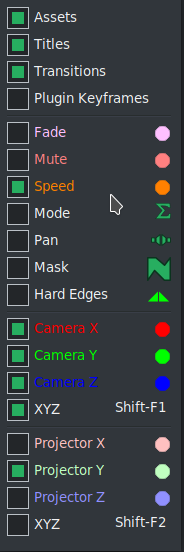
\includegraphics[width=0.99\linewidth]{images/overlays_list1.png}
        \caption{Original Settings --- cool spot}
        \label{fig:overlays_list1}
    \end{minipage}
    \hfill
    \begin{minipage}{.29\linewidth}
        \centering
        \includegraphics[width=0.99\linewidth]{images/overlays_list2.png}
        \caption{Note Titles box hot spot  }
        \label{fig:overlays_list2}
    \end{minipage}
    \hfill
    \begin{minipage}{.29\linewidth}
        \centering
        \includegraphics[width=0.99\linewidth]{images/overlays_list3.png}
        \caption{Cam/Proj XYZ toggle to fine tune}
        \label{fig:overlays_list3}
    \end{minipage}
\end{figure}


\subsection{Sound Level Meters Window}%
\label{sub:sound_level_meters_window}

An additional window, the levels window, can be brought up from the Window pulldown.  
The levels window displays the output audio levels after all mixing is done.  
The visible range of the sound level meters is configurable in Settings$\rightarrow$Preferences, Interface tab under the Operations section.

\begin{wrapfigure}[16]{O}{0.3\linewidth} 
    \centering
    %\vspace{-4ex}
    \includegraphics[width=0.5\linewidth]{images/volume_meter.png}
    \caption{Sound Level Meters Window}
    \label{fig:volume_meter}
\end{wrapfigure}

Sound level meters can be toggled in the viewer and compositor windows with the show meters button.  
They also appear in the patchbay when the track is expanded and in the recording monitor when audio is being recorded. 

The sound levels in the levels window, compositor, and viewer correspond to the final output levels before they are clipped to the sound card range.  
In the record monitor they are the input values from the sound card.  
In the patchbay they are the sound levels for each track after all effects are processed and before down-mixing for the output.  
Most of the time, audio levels have numerical markings in dB but in the patchbay there is not enough room.



The sound level is color coded as an extra means of determining the sound level.  
Even without numerical markings, the sound level color can distinguish between several ranges and overload.  
Look at the color codings in a meter with numerical markings to see what colors correspond to what sound level.  
Then for meters in the patchbay in expanded audio tracks, use the color codings to see if it is overloading.

Be aware that sound levels in Cinelerra can go above 0 dB.  
This allows for not only seeing if a track is overloading but how much information is being lost by the overloading.  
Overloading by less than 3 dB is usually acceptable.  
While overloading is treated as positive numbers in Cinelerra, it is clipped to 0 when sent to a sound card or file.







